\documentclass[]{book}
\usepackage{lmodern}
\usepackage{amssymb,amsmath}
\usepackage{ifxetex,ifluatex}
\usepackage{fixltx2e} % provides \textsubscript
\ifnum 0\ifxetex 1\fi\ifluatex 1\fi=0 % if pdftex
  \usepackage[T1]{fontenc}
  \usepackage[utf8]{inputenc}
\else % if luatex or xelatex
  \ifxetex
    \usepackage{mathspec}
  \else
    \usepackage{fontspec}
  \fi
  \defaultfontfeatures{Ligatures=TeX,Scale=MatchLowercase}
\fi
% use upquote if available, for straight quotes in verbatim environments
\IfFileExists{upquote.sty}{\usepackage{upquote}}{}
% use microtype if available
\IfFileExists{microtype.sty}{%
\usepackage{microtype}
\UseMicrotypeSet[protrusion]{basicmath} % disable protrusion for tt fonts
}{}
\usepackage[margin=1in]{geometry}
\usepackage{hyperref}
\hypersetup{unicode=true,
            pdftitle={Time Series and Longitudinal Analysis},
            pdfauthor={Richard White},
            pdfborder={0 0 0},
            breaklinks=true}
\urlstyle{same}  % don't use monospace font for urls
\usepackage{natbib}
\bibliographystyle{apalike}
\usepackage{color}
\usepackage{fancyvrb}
\newcommand{\VerbBar}{|}
\newcommand{\VERB}{\Verb[commandchars=\\\{\}]}
\DefineVerbatimEnvironment{Highlighting}{Verbatim}{commandchars=\\\{\}}
% Add ',fontsize=\small' for more characters per line
\usepackage{framed}
\definecolor{shadecolor}{RGB}{248,248,248}
\newenvironment{Shaded}{\begin{snugshade}}{\end{snugshade}}
\newcommand{\KeywordTok}[1]{\textcolor[rgb]{0.13,0.29,0.53}{\textbf{#1}}}
\newcommand{\DataTypeTok}[1]{\textcolor[rgb]{0.13,0.29,0.53}{#1}}
\newcommand{\DecValTok}[1]{\textcolor[rgb]{0.00,0.00,0.81}{#1}}
\newcommand{\BaseNTok}[1]{\textcolor[rgb]{0.00,0.00,0.81}{#1}}
\newcommand{\FloatTok}[1]{\textcolor[rgb]{0.00,0.00,0.81}{#1}}
\newcommand{\ConstantTok}[1]{\textcolor[rgb]{0.00,0.00,0.00}{#1}}
\newcommand{\CharTok}[1]{\textcolor[rgb]{0.31,0.60,0.02}{#1}}
\newcommand{\SpecialCharTok}[1]{\textcolor[rgb]{0.00,0.00,0.00}{#1}}
\newcommand{\StringTok}[1]{\textcolor[rgb]{0.31,0.60,0.02}{#1}}
\newcommand{\VerbatimStringTok}[1]{\textcolor[rgb]{0.31,0.60,0.02}{#1}}
\newcommand{\SpecialStringTok}[1]{\textcolor[rgb]{0.31,0.60,0.02}{#1}}
\newcommand{\ImportTok}[1]{#1}
\newcommand{\CommentTok}[1]{\textcolor[rgb]{0.56,0.35,0.01}{\textit{#1}}}
\newcommand{\DocumentationTok}[1]{\textcolor[rgb]{0.56,0.35,0.01}{\textbf{\textit{#1}}}}
\newcommand{\AnnotationTok}[1]{\textcolor[rgb]{0.56,0.35,0.01}{\textbf{\textit{#1}}}}
\newcommand{\CommentVarTok}[1]{\textcolor[rgb]{0.56,0.35,0.01}{\textbf{\textit{#1}}}}
\newcommand{\OtherTok}[1]{\textcolor[rgb]{0.56,0.35,0.01}{#1}}
\newcommand{\FunctionTok}[1]{\textcolor[rgb]{0.00,0.00,0.00}{#1}}
\newcommand{\VariableTok}[1]{\textcolor[rgb]{0.00,0.00,0.00}{#1}}
\newcommand{\ControlFlowTok}[1]{\textcolor[rgb]{0.13,0.29,0.53}{\textbf{#1}}}
\newcommand{\OperatorTok}[1]{\textcolor[rgb]{0.81,0.36,0.00}{\textbf{#1}}}
\newcommand{\BuiltInTok}[1]{#1}
\newcommand{\ExtensionTok}[1]{#1}
\newcommand{\PreprocessorTok}[1]{\textcolor[rgb]{0.56,0.35,0.01}{\textit{#1}}}
\newcommand{\AttributeTok}[1]{\textcolor[rgb]{0.77,0.63,0.00}{#1}}
\newcommand{\RegionMarkerTok}[1]{#1}
\newcommand{\InformationTok}[1]{\textcolor[rgb]{0.56,0.35,0.01}{\textbf{\textit{#1}}}}
\newcommand{\WarningTok}[1]{\textcolor[rgb]{0.56,0.35,0.01}{\textbf{\textit{#1}}}}
\newcommand{\AlertTok}[1]{\textcolor[rgb]{0.94,0.16,0.16}{#1}}
\newcommand{\ErrorTok}[1]{\textcolor[rgb]{0.64,0.00,0.00}{\textbf{#1}}}
\newcommand{\NormalTok}[1]{#1}
\usepackage{longtable,booktabs}
\usepackage{graphicx,grffile}
\makeatletter
\def\maxwidth{\ifdim\Gin@nat@width>\linewidth\linewidth\else\Gin@nat@width\fi}
\def\maxheight{\ifdim\Gin@nat@height>\textheight\textheight\else\Gin@nat@height\fi}
\makeatother
% Scale images if necessary, so that they will not overflow the page
% margins by default, and it is still possible to overwrite the defaults
% using explicit options in \includegraphics[width, height, ...]{}
\setkeys{Gin}{width=\maxwidth,height=\maxheight,keepaspectratio}
\IfFileExists{parskip.sty}{%
\usepackage{parskip}
}{% else
\setlength{\parindent}{0pt}
\setlength{\parskip}{6pt plus 2pt minus 1pt}
}
\setlength{\emergencystretch}{3em}  % prevent overfull lines
\providecommand{\tightlist}{%
  \setlength{\itemsep}{0pt}\setlength{\parskip}{0pt}}
\setcounter{secnumdepth}{5}
% Redefines (sub)paragraphs to behave more like sections
\ifx\paragraph\undefined\else
\let\oldparagraph\paragraph
\renewcommand{\paragraph}[1]{\oldparagraph{#1}\mbox{}}
\fi
\ifx\subparagraph\undefined\else
\let\oldsubparagraph\subparagraph
\renewcommand{\subparagraph}[1]{\oldsubparagraph{#1}\mbox{}}
\fi

%%% Use protect on footnotes to avoid problems with footnotes in titles
\let\rmarkdownfootnote\footnote%
\def\footnote{\protect\rmarkdownfootnote}

%%% Change title format to be more compact
\usepackage{titling}

% Create subtitle command for use in maketitle
\newcommand{\subtitle}[1]{
  \posttitle{
    \begin{center}\large#1\end{center}
    }
}

\setlength{\droptitle}{-2em}

  \title{Time Series and Longitudinal Analysis}
    \pretitle{\vspace{\droptitle}\centering\huge}
  \posttitle{\par}
    \author{Richard White}
    \preauthor{\centering\large\emph}
  \postauthor{\par}
      \predate{\centering\large\emph}
  \postdate{\par}
    \date{2018-11-08}

\usepackage{booktabs}

\begin{document}
\maketitle

{
\setcounter{tocdepth}{1}
\tableofcontents
}
\chapter*{Preface}\label{preface}
\addcontentsline{toc}{chapter}{Preface}

When dealing with data measured over time, there are two kinds of
analyses that can be performed.

``Time series'' analyses generally deal with one variable (the outcome).
We can then either:

\begin{enumerate}
\def\labelenumi{\arabic{enumi}.}
\tightlist
\item
  Predict the future only using the previous observations. E.g. predict
  tomorrow's temperature, using today's and yesterday's temperature as
  exposures. We will not be focusing on these kinds of analyses.
\item
  Estimate descriptive statistics about the data. E.g. Today's data is
  much higher than expected (outbreak?). We will focus on these kinds of
  analyses.
\end{enumerate}

If we have more than one variable measured over time (e.g.~outcome and
an exposure) then we can run regression analyses. E.g. seeing how the
number of tuberculosis patients (outcome) is affected by the number of
immigrants to Norway (exposure) over a 20 year period. We will focus on
these kinds of analyses.

It is important to note that if we define our exposure as ``time'' then
we can use the regression framework to estimate descriptive statistics
about the data. This means we can use the same regression framework for
the two kinds of analyses we will be focusing on.

The ``regression framework'' is very similar to ordinary regressions
that you have been working with for many years. The only difference is
that some of the data \textbf{may} have more advanced data structures
that your normal methods cannot handle.

\chapter{Definitions and Scenarios}\label{definitions-and-scenarios}

\section{Panel Data}\label{panel-data}

Panel data is a set of data with measurements repeated at equally spaced
points. For example, number of influenza cases recorded every day, or
every week, or every year would be considered panel data. The number of
influenza cases on Jan 31, Feb 3, and Nov 21 in 2018 would not be
considered panel data.

\section{Autocorrelation}\label{autocorrelation}

When you have panel data, autocorrelation is the correlation between
subsequent observations. For example, if you have daily observations,
then the 1 day autocorrelation is the correlation between observations 1
day apart, and likewise the 2 day autocorrelation is the correlation
between observations 2 days apart.

\section{Scenarios}\label{scenarios}

In this course we will consider two scenarios where we have multiple
observations for each geographical area:

\begin{itemize}
\tightlist
\item
  Panel data: One geographical area with/without autocorrelation
\item
  Panel data: Multiple geographical areas without autocorrelation
\end{itemize}

Note, the following scenario can be covered by standard regression
models:

\begin{itemize}
\tightlist
\item
  Multiple geographical areas, one time point/observation per
  geographical area
\end{itemize}

\section{Useful Code}\label{useful-code}

This code is used to calculate prediction intervals. In its most basic
form it is:

\[
95\% \text{ prediction interval} = \text{sample average} \pm 1.96 \times \text{sample standard deviation} \sqrt{ 1 + 1 / n}
\] However, due to the skewness of the count data, we often choose to
use a \texttt{2/3s\ transformation}.

\begin{Shaded}
\begin{Highlighting}[]
\NormalTok{sykdomspuls}\OperatorTok{::}\NormalTok{FarringtonThreshold}
\end{Highlighting}
\end{Shaded}

\begin{verbatim}
## function (pred, phi, alpha = NULL, z = NULL, skewness.transform = "none") 
## {
##     mu0 <- pred$fit
##     tau <- phi + (pred$se.fit^2)/mu0
##     switch(skewness.transform, none = {
##         se <- sqrt(mu0 * tau)
##         exponent <- 1
##     }, `1/2` = {
##         se <- sqrt(1/4 * tau)
##         exponent <- 1/2
##     }, `2/3` = {
##         se <- sqrt(4/9 * mu0^(1/3) * tau)
##         exponent <- 2/3
##     }, {
##         stop("No proper exponent in algo.farrington.threshold.")
##     })
##     if (is.null(z)) 
##         z <- qnorm(1 - alpha/2)
##     lu <- (mu0^exponent + z * se)^(1/exponent)
##     return(lu)
## }
## <bytecode: 0x4080170>
## <environment: namespace:sykdomspuls>
\end{verbatim}

Please note that a prediction interval is not the same as a confidence
interval!

\chapter{Panel Data - One Area}\label{panel-data---one-area}

\section{Aim}\label{aim}

We are given a dataset containing daily counts of diseases from one
geographical area. We want to identify:

\begin{enumerate}
\def\labelenumi{\arabic{enumi}.}
\tightlist
\item
  Does seasonality exist?
\item
  If seasonality exists, when are the high/low seasons?
\item
  Is there a general yearly trend (i.e.~increasing or decreasing from
  year to year?)
\item
  Is daily rainfall associated with the number of cases?
\item
  When are there outbreaks?
\end{enumerate}

\begin{Shaded}
\begin{Highlighting}[]
\KeywordTok{library}\NormalTok{(data.table)}
\KeywordTok{library}\NormalTok{(ggplot2)}
\KeywordTok{set.seed}\NormalTok{(}\DecValTok{4}\NormalTok{)}

\NormalTok{AMPLITUDE <-}\StringTok{ }\FloatTok{1.5}
\NormalTok{SEASONAL_HORIZONTAL_SHIFT <-}\StringTok{ }\DecValTok{20}

\NormalTok{d <-}\StringTok{ }\KeywordTok{data.table}\NormalTok{(}\DataTypeTok{date =} \KeywordTok{seq.Date}\NormalTok{(}
  \DataTypeTok{from =} \KeywordTok{as.Date}\NormalTok{(}\StringTok{"2000-01-01"}\NormalTok{),}
  \DataTypeTok{to =} \KeywordTok{as.Date}\NormalTok{(}\StringTok{"2018-12-31"}\NormalTok{),}
  \DataTypeTok{by =} \DecValTok{1}
\NormalTok{))}
\NormalTok{d[, date }\OperatorTok{:}\ErrorTok{=}\StringTok{ }\KeywordTok{as.Date}\NormalTok{(date, }\DataTypeTok{origin =} \StringTok{"1970-01-1"}\NormalTok{)]}
\NormalTok{d[, year }\OperatorTok{:}\ErrorTok{=}\StringTok{ }\KeywordTok{as.numeric}\NormalTok{(}\KeywordTok{format.Date}\NormalTok{(date, }\StringTok{"%G"}\NormalTok{))]}
\NormalTok{d[, week }\OperatorTok{:}\ErrorTok{=}\StringTok{ }\KeywordTok{as.numeric}\NormalTok{(}\KeywordTok{format.Date}\NormalTok{(date, }\StringTok{"%V"}\NormalTok{))]}
\NormalTok{d[, month }\OperatorTok{:}\ErrorTok{=}\StringTok{ }\KeywordTok{as.numeric}\NormalTok{(}\KeywordTok{format.Date}\NormalTok{(date, }\StringTok{"%m"}\NormalTok{))]}
\NormalTok{d[, yearMinus2000 }\OperatorTok{:}\ErrorTok{=}\StringTok{ }\NormalTok{year }\OperatorTok{-}\StringTok{ }\DecValTok{2000}\NormalTok{]}
\NormalTok{d[, dailyrainfall }\OperatorTok{:}\ErrorTok{=}\StringTok{ }\KeywordTok{runif}\NormalTok{(.N, }\DataTypeTok{min =} \DecValTok{0}\NormalTok{, }\DataTypeTok{max =} \DecValTok{10}\NormalTok{)]}

\NormalTok{d[, dayOfYear }\OperatorTok{:}\ErrorTok{=}\StringTok{ }\KeywordTok{as.numeric}\NormalTok{(}\KeywordTok{format.Date}\NormalTok{(date, }\StringTok{"%j"}\NormalTok{))]}
\NormalTok{d[, seasonalEffect }\OperatorTok{:}\ErrorTok{=}\StringTok{ }\KeywordTok{sin}\NormalTok{(}\DecValTok{2} \OperatorTok{*}\StringTok{ }\NormalTok{pi }\OperatorTok{*}\StringTok{ }\NormalTok{(dayOfYear }\OperatorTok{-}\StringTok{ }\NormalTok{SEASONAL_HORIZONTAL_SHIFT) }\OperatorTok{/}\StringTok{ }\DecValTok{365}\NormalTok{)]}
\NormalTok{d[, mu }\OperatorTok{:}\ErrorTok{=}\StringTok{ }\KeywordTok{exp}\NormalTok{(}\FloatTok{0.1} \OperatorTok{+}\StringTok{ }\NormalTok{yearMinus2000 }\OperatorTok{*}\StringTok{ }\FloatTok{0.1} \OperatorTok{+}\StringTok{ }\NormalTok{seasonalEffect }\OperatorTok{*}\StringTok{ }\NormalTok{AMPLITUDE)]}
\NormalTok{d[, y }\OperatorTok{:}\ErrorTok{=}\StringTok{ }\KeywordTok{rpois}\NormalTok{(.N, mu)]}
\end{Highlighting}
\end{Shaded}

\section{Data}\label{data}

Here we show the true data, and note that there is an increasing annual
trend (the data gets higher as time goes on) and there is a seasonal
pattern (one peak/trough per year)

\begin{Shaded}
\begin{Highlighting}[]
\NormalTok{q <-}\StringTok{ }\KeywordTok{ggplot}\NormalTok{(d, }\KeywordTok{aes}\NormalTok{(}\DataTypeTok{x =}\NormalTok{ date, }\DataTypeTok{y =}\NormalTok{ y))}
\NormalTok{q <-}\StringTok{ }\NormalTok{q }\OperatorTok{+}\StringTok{ }\KeywordTok{geom_line}\NormalTok{(}\DataTypeTok{lwd =} \FloatTok{0.25}\NormalTok{)}
\NormalTok{q <-}\StringTok{ }\NormalTok{q }\OperatorTok{+}\StringTok{ }\KeywordTok{scale_x_date}\NormalTok{(}\StringTok{"Time"}\NormalTok{)}
\NormalTok{q <-}\StringTok{ }\NormalTok{q }\OperatorTok{+}\StringTok{ }\KeywordTok{scale_y_continuous}\NormalTok{(}\StringTok{"Cases"}\NormalTok{)}
\NormalTok{q}
\end{Highlighting}
\end{Shaded}

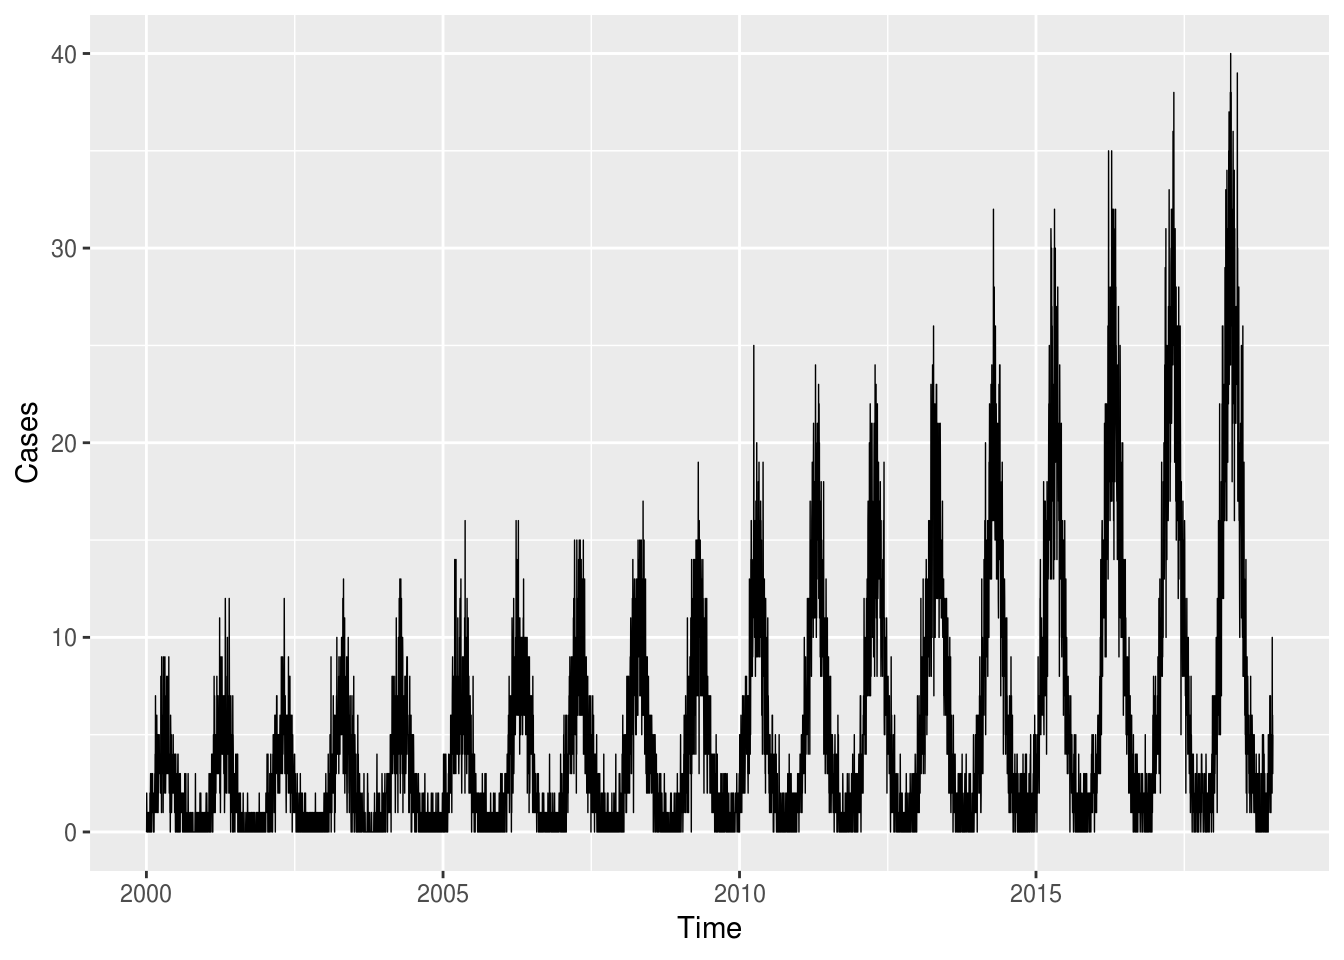
\includegraphics{website_files/figure-latex/unnamed-chunk-3-1.pdf}

We split out the data for a few years and see a clear seasonal trend:

\begin{Shaded}
\begin{Highlighting}[]
\NormalTok{q <-}\StringTok{ }\KeywordTok{ggplot}\NormalTok{(d[year }\OperatorTok\StringTok{ }\KeywordTok{c}\NormalTok{(}\DecValTok{2005}\OperatorTok{:}\DecValTok{2010}\NormalTok{)], }\KeywordTok{aes}\NormalTok{(}\DataTypeTok{x =}\NormalTok{ dayOfYear, }\DataTypeTok{y =}\NormalTok{ y))}
\NormalTok{q <-}\StringTok{ }\NormalTok{q }\OperatorTok{+}\StringTok{ }\KeywordTok{facet_wrap}\NormalTok{(}\OperatorTok{~}\NormalTok{year)}
\NormalTok{q <-}\StringTok{ }\NormalTok{q }\OperatorTok{+}\StringTok{ }\KeywordTok{geom_point}\NormalTok{()}
\NormalTok{q <-}\StringTok{ }\NormalTok{q }\OperatorTok{+}\StringTok{ }\KeywordTok{stat_smooth}\NormalTok{(}\DataTypeTok{colour =} \StringTok{"red"}\NormalTok{)}
\NormalTok{q <-}\StringTok{ }\NormalTok{q }\OperatorTok{+}\StringTok{ }\KeywordTok{scale_x_continuous}\NormalTok{(}\StringTok{"Day of year"}\NormalTok{)}
\NormalTok{q <-}\StringTok{ }\NormalTok{q }\OperatorTok{+}\StringTok{ }\KeywordTok{scale_y_continuous}\NormalTok{(}\StringTok{"Cases"}\NormalTok{)}
\NormalTok{q}
\end{Highlighting}
\end{Shaded}

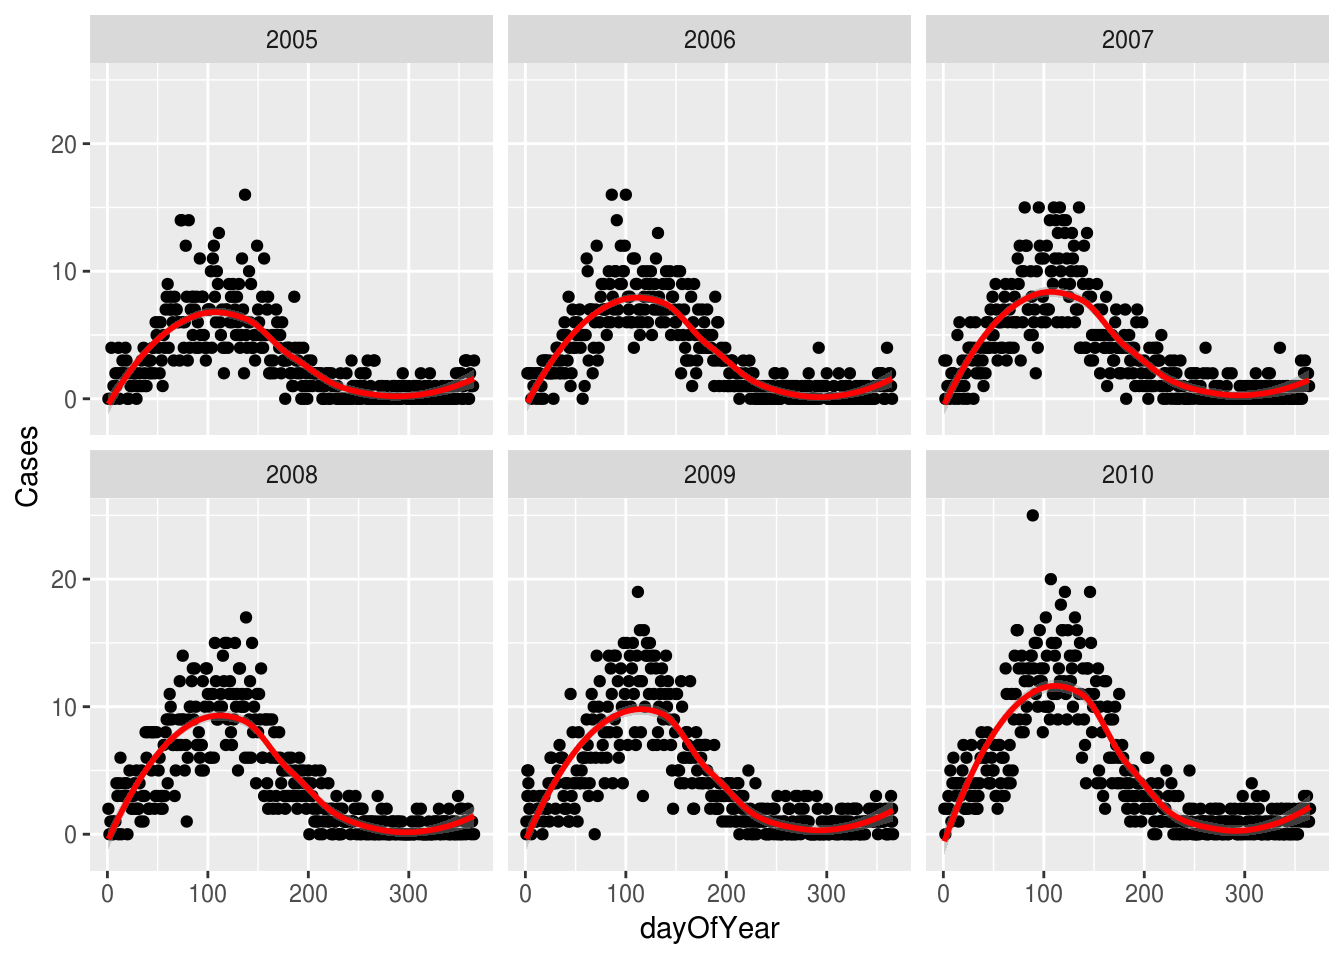
\includegraphics{website_files/figure-latex/unnamed-chunk-4-1.pdf}

\section{Model With Non-Parametric
Seasonality}\label{model-with-non-parametric-seasonality}

If we want to investigate the seasonality of our data, and identify when
are the peaks and troughs, we can use non-parametric approaches. They
are flexible and easy to implement, but they can lack power and be hard
to interpret:

\begin{itemize}
\tightlist
\item
  Create a categorical variable for the seasons (e.g. \texttt{spring},
  \texttt{summer}, \texttt{autumn}, \texttt{winter}) and include this in
  the regression model
\item
  Create a categorical variable for the months (e.g. \texttt{Jan},
  \texttt{Feb}, \ldots{}, \texttt{Dec}) and include this in the
  regression model
\end{itemize}

\begin{Shaded}
\begin{Highlighting}[]
\NormalTok{nfit0 <-}\StringTok{ }\KeywordTok{glm}\NormalTok{(y }\OperatorTok{~}\StringTok{ }\NormalTok{yearMinus2000 }\OperatorTok{+}\StringTok{ }\NormalTok{dailyrainfall, }\DataTypeTok{data =}\NormalTok{ d, }\DataTypeTok{family =} \KeywordTok{poisson}\NormalTok{())}
\NormalTok{nfit1 <-}\StringTok{ }\KeywordTok{glm}\NormalTok{(y }\OperatorTok{~}\StringTok{ }\NormalTok{yearMinus2000 }\OperatorTok{+}\StringTok{ }\NormalTok{dailyrainfall }\OperatorTok{+}\StringTok{ }\KeywordTok{as.factor}\NormalTok{(month), }\DataTypeTok{data =}\NormalTok{ d, }\DataTypeTok{family =} \KeywordTok{poisson}\NormalTok{())}
\end{Highlighting}
\end{Shaded}

\subsection{Seasonality}\label{seasonality}

We can test the \texttt{month} categorical variable using a likelihood
ratio test:

\begin{Shaded}
\begin{Highlighting}[]
\NormalTok{lmtest}\OperatorTok{::}\KeywordTok{lrtest}\NormalTok{(nfit0, nfit1)}
\end{Highlighting}
\end{Shaded}

\begin{verbatim}
## Likelihood ratio test
## 
## Model 1: y ~ yearMinus2000 + dailyrainfall
## Model 2: y ~ yearMinus2000 + dailyrainfall + as.factor(month)
##   #Df LogLik Df Chisq Pr(>Chisq)    
## 1   3 -26904                        
## 2  14 -13251 11 27307  < 2.2e-16 ***
## ---
## Signif. codes:  0 '***' 0.001 '**' 0.01 '*' 0.05 '.' 0.1 ' ' 1
\end{verbatim}

\textbf{Question 1:} Does seasonality exist?

And then we can look at the output of our regression:

\begin{Shaded}
\begin{Highlighting}[]
\KeywordTok{summary}\NormalTok{(nfit1)}
\end{Highlighting}
\end{Shaded}

\begin{verbatim}
## 
## Call:
## glm(formula = y ~ yearMinus2000 + dailyrainfall + as.factor(month), 
##     family = poisson(), data = d)
## 
## Deviance Residuals: 
##     Min       1Q   Median       3Q      Max  
## -4.2874  -0.9578  -0.1498   0.5894   3.9130  
## 
## Coefficients:
##                     Estimate Std. Error z value Pr(>|z|)    
## (Intercept)        -0.003849   0.028882  -0.133    0.894    
## yearMinus2000       0.101654   0.001053  96.578   <2e-16 ***
## dailyrainfall       0.000442   0.001852   0.239    0.811    
## as.factor(month)2   0.751048   0.029854  25.157   <2e-16 ***
## as.factor(month)3   1.303525   0.027328  47.700   <2e-16 ***
## as.factor(month)4   1.543098   0.026781  57.619   <2e-16 ***
## as.factor(month)5   1.425207   0.026992  52.801   <2e-16 ***
## as.factor(month)6   0.955465   0.028647  33.354   <2e-16 ***
## as.factor(month)7   0.286169   0.032060   8.926   <2e-16 ***
## as.factor(month)8  -0.541443   0.039932 -13.559   <2e-16 ***
## as.factor(month)9  -1.114005   0.049322 -22.586   <2e-16 ***
## as.factor(month)10 -1.350683   0.053389 -25.299   <2e-16 ***
## as.factor(month)11 -1.235671   0.051682 -23.909   <2e-16 ***
## as.factor(month)12 -0.754107   0.042777 -17.629   <2e-16 ***
## ---
## Signif. codes:  0 '***' 0.001 '**' 0.01 '*' 0.05 '.' 0.1 ' ' 1
## 
## (Dispersion parameter for poisson family taken to be 1)
## 
##     Null deviance: 45536.8  on 6939  degrees of freedom
## Residual deviance:  8045.6  on 6926  degrees of freedom
## AIC: 26529
## 
## Number of Fisher Scoring iterations: 5
\end{verbatim}

\emph{NOTE:} See that this is basically the same as a normal regression.

\textbf{Question 2:} If seasonality exists, when are the high/low
seasons?

\subsection{Yearly trend}\label{yearly-trend}

\textbf{Question 3:} Is there a general yearly trend (i.e.~increasing or
decreasing from year to year?)

\subsection{Association With Rainfall}\label{association-with-rainfall}

\textbf{Question 4:} Is daily rainfall associated with the number of
cases?

\subsection{Outbreaks}\label{outbreaks}

If we want to identify outbreaks, then we need to use the standard
prediction interval formula:

\[
95\% \text{ prediction interval} = \text{sample average} \pm 1.96 \times \text{sample standard deviation} \sqrt{ 1 + 1 / n}
\] This allows us to identify what the expected thresholds are:

\begin{Shaded}
\begin{Highlighting}[]
\NormalTok{pred <-}\StringTok{ }\KeywordTok{predict}\NormalTok{(nfit1, }\DataTypeTok{type =} \StringTok{"response"}\NormalTok{, }\DataTypeTok{se.fit =}\NormalTok{ T, }\DataTypeTok{newdata =}\NormalTok{ d)}
\NormalTok{d[, threshold0 }\OperatorTok{:}\ErrorTok{=}\StringTok{ }\NormalTok{pred}\OperatorTok{$}\NormalTok{fit]}
\NormalTok{d[, threshold2 }\OperatorTok{:}\ErrorTok{=}\StringTok{ }\NormalTok{sykdomspuls}\OperatorTok{::}\KeywordTok{FarringtonThreshold}\NormalTok{(pred, }\DataTypeTok{phi =} \DecValTok{1}\NormalTok{, }\DataTypeTok{z =} \DecValTok{2}\NormalTok{, }\DataTypeTok{skewness.transform =} \StringTok{"2/3"}\NormalTok{)]}
\end{Highlighting}
\end{Shaded}

\textbf{Question 5:} When are there outbreaks?

\begin{Shaded}
\begin{Highlighting}[]
\NormalTok{q <-}\StringTok{ }\KeywordTok{ggplot}\NormalTok{(d[year }\OperatorTok{>}\StringTok{ }\DecValTok{2015}\NormalTok{], }\KeywordTok{aes}\NormalTok{(}\DataTypeTok{x =}\NormalTok{ date, }\DataTypeTok{y =}\NormalTok{ y))}
\NormalTok{q <-}\StringTok{ }\NormalTok{q }\OperatorTok{+}\StringTok{ }\KeywordTok{geom_ribbon}\NormalTok{(}\DataTypeTok{mapping =} \KeywordTok{aes}\NormalTok{(}\DataTypeTok{ymin =} \OperatorTok{-}\OtherTok{Inf}\NormalTok{, }\DataTypeTok{ymax =}\NormalTok{ threshold2), }\DataTypeTok{fill =} \StringTok{"blue"}\NormalTok{, }\DataTypeTok{alpha =} \FloatTok{0.5}\NormalTok{)}
\NormalTok{q <-}\StringTok{ }\NormalTok{q }\OperatorTok{+}\StringTok{ }\KeywordTok{geom_ribbon}\NormalTok{(}\DataTypeTok{mapping =} \KeywordTok{aes}\NormalTok{(}\DataTypeTok{ymin =}\NormalTok{ threshold2, }\DataTypeTok{ymax =} \OtherTok{Inf}\NormalTok{), }\DataTypeTok{fill =} \StringTok{"red"}\NormalTok{, }\DataTypeTok{alpha =} \FloatTok{0.5}\NormalTok{)}
\NormalTok{q <-}\StringTok{ }\NormalTok{q }\OperatorTok{+}\StringTok{ }\KeywordTok{geom_line}\NormalTok{(}\DataTypeTok{lwd =} \FloatTok{0.25}\NormalTok{)}
\NormalTok{q <-}\StringTok{ }\NormalTok{q }\OperatorTok{+}\StringTok{ }\KeywordTok{geom_point}\NormalTok{(}\DataTypeTok{data =}\NormalTok{ d[year }\OperatorTok{>}\StringTok{ }\DecValTok{2015} \OperatorTok{&}\StringTok{ }\NormalTok{y }\OperatorTok{>}\StringTok{ }\NormalTok{threshold2], }\DataTypeTok{colour =} \StringTok{"black"}\NormalTok{, }\DataTypeTok{size =} \FloatTok{2.5}\NormalTok{)}
\NormalTok{q <-}\StringTok{ }\NormalTok{q }\OperatorTok{+}\StringTok{ }\KeywordTok{geom_point}\NormalTok{(}\DataTypeTok{data =}\NormalTok{ d[year }\OperatorTok{>}\StringTok{ }\DecValTok{2015} \OperatorTok{&}\StringTok{ }\NormalTok{y }\OperatorTok{>}\StringTok{ }\NormalTok{threshold2], }\DataTypeTok{colour =} \StringTok{"red"}\NormalTok{, }\DataTypeTok{size =} \FloatTok{1.5}\NormalTok{)}
\NormalTok{q <-}\StringTok{ }\NormalTok{q }\OperatorTok{+}\StringTok{ }\KeywordTok{scale_x_date}\NormalTok{(}\StringTok{"Time"}\NormalTok{)}
\NormalTok{q <-}\StringTok{ }\NormalTok{q }\OperatorTok{+}\StringTok{ }\KeywordTok{scale_y_continuous}\NormalTok{(}\StringTok{"Cases"}\NormalTok{)}
\NormalTok{q}
\end{Highlighting}
\end{Shaded}

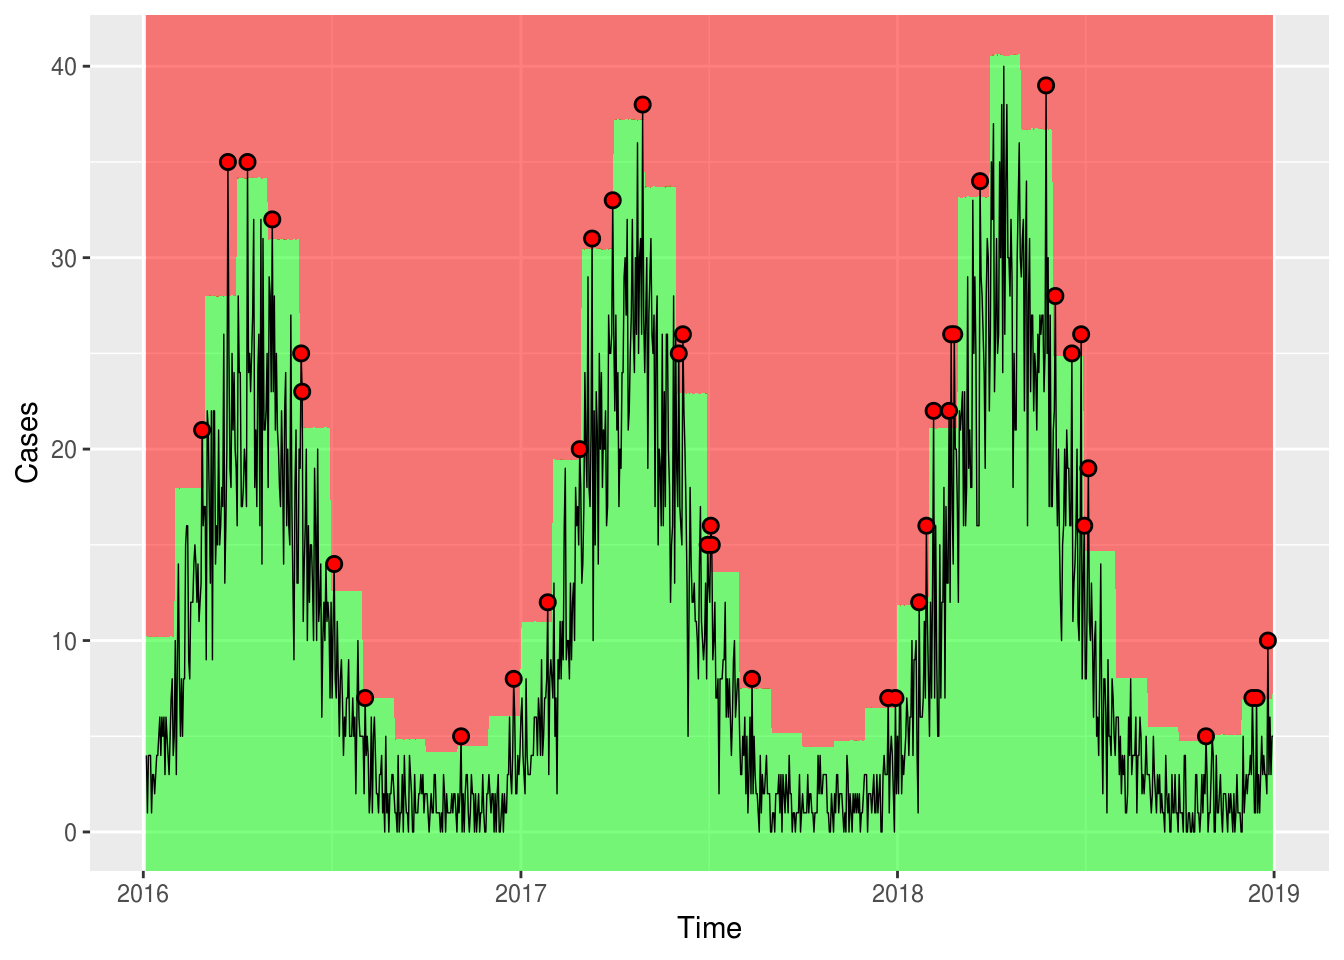
\includegraphics{website_files/figure-latex/unnamed-chunk-9-1.pdf}

\section{Model With Parametric
Seasonality}\label{model-with-parametric-seasonality}

Parametric approaches are more powerful but require more effort:

\begin{itemize}
\tightlist
\item
  Identify the periodicity of the seasonality (how many days between
  peaks?)
\item
  Using trigonometry, transform \texttt{day\ of\ year} into variables
  that appropriately model the observed periodicity
\item
  Obtain coefficient estimates
\item
  Back-transform these estimates into human-understandable values (day
  of peak, day of trough)
\end{itemize}

\emph{NOTE:} You don't always have to investigate seasonality! It
depends entirely on what the purpose of your analysis is!

\subsection{Seasonality}\label{seasonality-1}

The Lomb-Scargle Periodogram shows a clear seasonality with a period of
365 days.

\begin{Shaded}
\begin{Highlighting}[]
\CommentTok{# R CODE}
\NormalTok{lomb}\OperatorTok{::}\KeywordTok{lsp}\NormalTok{(d}\OperatorTok{$}\NormalTok{y, }\DataTypeTok{from =} \DecValTok{100}\NormalTok{, }\DataTypeTok{to =} \DecValTok{500}\NormalTok{, }\DataTypeTok{ofac =} \DecValTok{1}\NormalTok{, }\DataTypeTok{type =} \StringTok{"period"}\NormalTok{)}
\end{Highlighting}
\end{Shaded}

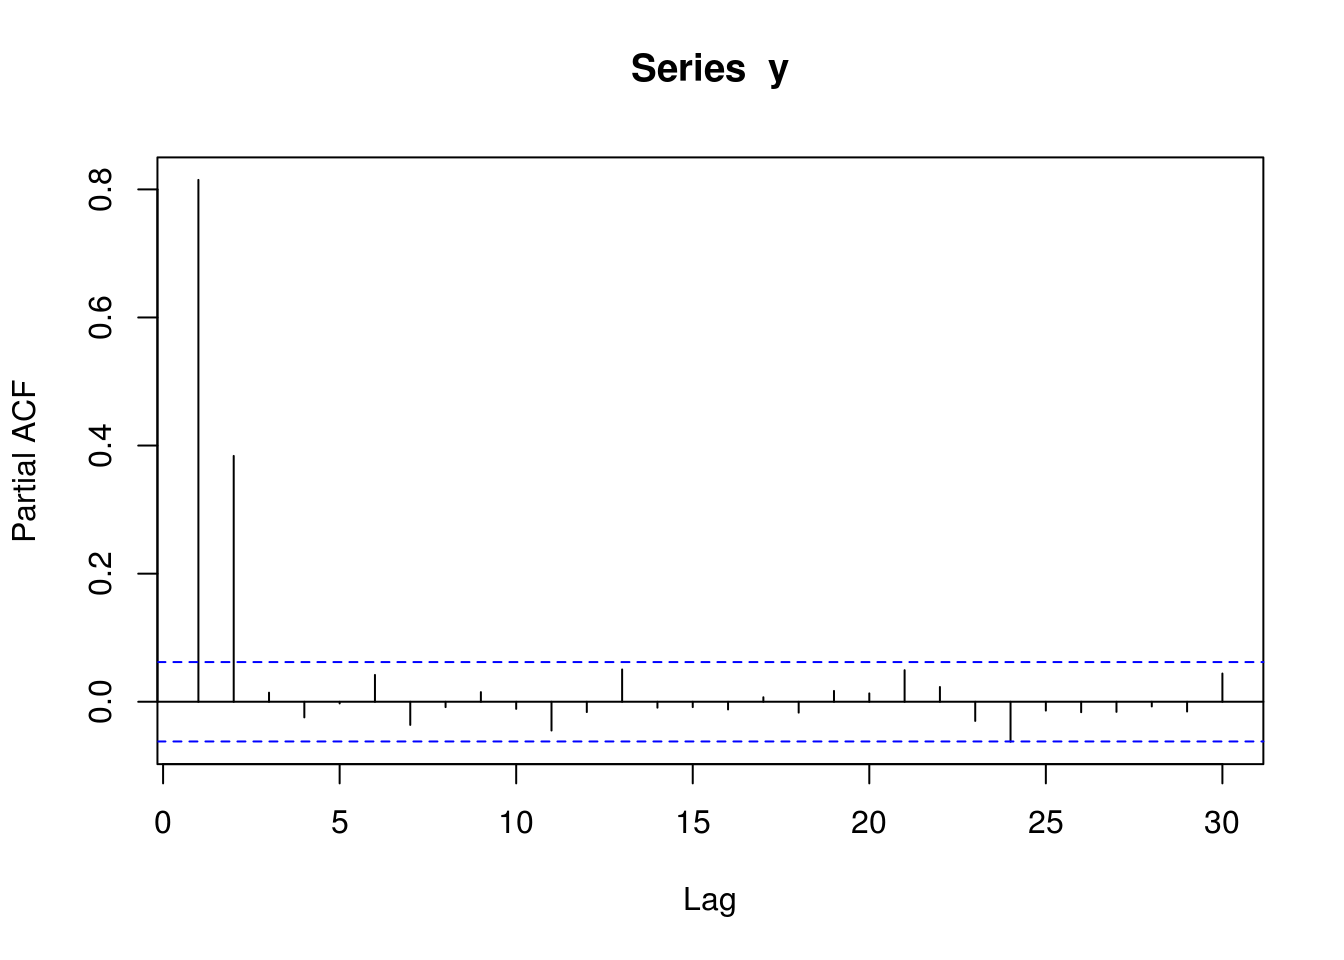
\includegraphics{website_files/figure-latex/unnamed-chunk-10-1.pdf}

We then generate two new variables \texttt{cos365} and \texttt{sin365}
and perform a likelihood ratio test to see if they are significant or
not. This is done with two simple poisson regressions.

\begin{Shaded}
\begin{Highlighting}[]
\CommentTok{# R CODE}
\NormalTok{d[, cos365 }\OperatorTok{:}\ErrorTok{=}\StringTok{ }\KeywordTok{cos}\NormalTok{(dayOfYear }\OperatorTok{*}\StringTok{ }\DecValTok{2} \OperatorTok{*}\StringTok{ }\NormalTok{pi }\OperatorTok{/}\StringTok{ }\DecValTok{365}\NormalTok{)]}
\NormalTok{d[, sin365 }\OperatorTok{:}\ErrorTok{=}\StringTok{ }\KeywordTok{sin}\NormalTok{(dayOfYear }\OperatorTok{*}\StringTok{ }\DecValTok{2} \OperatorTok{*}\StringTok{ }\NormalTok{pi }\OperatorTok{/}\StringTok{ }\DecValTok{365}\NormalTok{)]}

\NormalTok{pfit0 <-}\StringTok{ }\KeywordTok{glm}\NormalTok{(y }\OperatorTok{~}\StringTok{ }\NormalTok{yearMinus2000 }\OperatorTok{+}\StringTok{ }\NormalTok{dailyrainfall, }\DataTypeTok{data =}\NormalTok{ d, }\DataTypeTok{family =} \KeywordTok{poisson}\NormalTok{())}
\NormalTok{pfit1 <-}\StringTok{ }\KeywordTok{glm}\NormalTok{(y }\OperatorTok{~}\StringTok{ }\NormalTok{yearMinus2000 }\OperatorTok{+}\StringTok{ }\NormalTok{dailyrainfall }\OperatorTok{+}\StringTok{ }\NormalTok{sin365 }\OperatorTok{+}\StringTok{ }\NormalTok{cos365, }\DataTypeTok{data =}\NormalTok{ d, }\DataTypeTok{family =} \KeywordTok{poisson}\NormalTok{())}
\end{Highlighting}
\end{Shaded}

We can test the seasonality using a likelihood ratio test (which we
already strongly suspected due to the periodogram):

\begin{Shaded}
\begin{Highlighting}[]
\NormalTok{lmtest}\OperatorTok{::}\KeywordTok{lrtest}\NormalTok{(pfit0, pfit1)}
\end{Highlighting}
\end{Shaded}

\begin{verbatim}
## Likelihood ratio test
## 
## Model 1: y ~ yearMinus2000 + dailyrainfall
## Model 2: y ~ yearMinus2000 + dailyrainfall + sin365 + cos365
##   #Df LogLik Df Chisq Pr(>Chisq)    
## 1   3 -26904                        
## 2   5 -12892  2 28024  < 2.2e-16 ***
## ---
## Signif. codes:  0 '***' 0.001 '**' 0.01 '*' 0.05 '.' 0.1 ' ' 1
\end{verbatim}

\textbf{Question 1:} Does seasonality exist?

And then we can look at the output of our regression:

\begin{Shaded}
\begin{Highlighting}[]
\KeywordTok{summary}\NormalTok{(pfit1)}
\end{Highlighting}
\end{Shaded}

\begin{verbatim}
## 
## Call:
## glm(formula = y ~ yearMinus2000 + dailyrainfall + sin365 + cos365, 
##     family = poisson(), data = d)
## 
## Deviance Residuals: 
##     Min       1Q   Median       3Q      Max  
## -4.0676  -0.9229  -0.1170   0.5861   3.4103  
## 
## Coefficients:
##                 Estimate Std. Error z value Pr(>|z|)    
## (Intercept)    0.0887436  0.0176742   5.021 5.14e-07 ***
## yearMinus2000  0.1016117  0.0010525  96.539  < 2e-16 ***
## dailyrainfall  0.0002287  0.0018476   0.124    0.901    
## sin365         1.3972586  0.0103200 135.393  < 2e-16 ***
## cos365        -0.5035265  0.0086308 -58.341  < 2e-16 ***
## ---
## Signif. codes:  0 '***' 0.001 '**' 0.01 '*' 0.05 '.' 0.1 ' ' 1
## 
## (Dispersion parameter for poisson family taken to be 1)
## 
##     Null deviance: 45536.8  on 6939  degrees of freedom
## Residual deviance:  7328.5  on 6935  degrees of freedom
## AIC: 25794
## 
## Number of Fisher Scoring iterations: 5
\end{verbatim}

We also see that the (significant!) coefficient for \texttt{year} is
\texttt{0.1} which means that for each additional year, the outcome
increases by \texttt{exp(0.1)=1.11}. We also see that the coefficient
for \texttt{dailyrainfall} was not significant, which means that we did
not find a significant association between the outcome and
\texttt{dailyrainfall}.

\emph{NOTE:} See that this is basically the same as a normal regression.

Through the likelihood ratio test we saw a clear significant seasonal
effect. We can now use trigonometry to back-calculate the amplitude and
location of peak/troughs from the \texttt{cos365} and \texttt{sin365}
estimates:

\begin{Shaded}
\begin{Highlighting}[]
\NormalTok{RAWmisc}\OperatorTok{::}\NormalTok{TransformCosSinToAmplitudePeakTrough}
\end{Highlighting}
\end{Shaded}

\begin{verbatim}
## function (cos_b, sin_b) 
## {
##     b1 <- sin_b
##     b2 <- cos_b
##     amplitude <- sqrt(b1^2 + b2^2)
##     p <- atan(b1/b2) * 366/2/pi
##     if (p > 0) {
##         peak <- p
##         trough <- p + 366/2
##     }
##     else {
##         peak <- p + 366/2
##         trough <- p + 366
##     }
##     if (b1 < 0) {
##         g <- peak
##         peak <- trough
##         trough <- g
##     }
##     return(list(amplitude = amplitude, peak = peak, trough = trough))
## }
## <bytecode: 0x47ea6b8>
## <environment: namespace:RAWmisc>
\end{verbatim}

\begin{Shaded}
\begin{Highlighting}[]
\NormalTok{retval <-}\StringTok{ }\NormalTok{RAWmisc}\OperatorTok{::}\KeywordTok{TransformCosSinToAmplitudePeakTrough}\NormalTok{(}
  \DataTypeTok{cos_b =} \OperatorTok{-}\FloatTok{0.512912}\NormalTok{, }\CommentTok{# cos coefficient}
  \DataTypeTok{sin_b =} \FloatTok{1.428417} \CommentTok{# sin coefficient}
\NormalTok{)}

\KeywordTok{print}\NormalTok{(}\KeywordTok{sprintf}\NormalTok{(}\StringTok{"amplitude is estimated as %s"}\NormalTok{, }\KeywordTok{round}\NormalTok{(retval}\OperatorTok{$}\NormalTok{amplitude, }\DecValTok{2}\NormalTok{)))}
\end{Highlighting}
\end{Shaded}

\begin{verbatim}
## [1] "amplitude is estimated as 1.52"
\end{verbatim}

\begin{Shaded}
\begin{Highlighting}[]
\KeywordTok{print}\NormalTok{(}\KeywordTok{sprintf}\NormalTok{(}\StringTok{"peak is estimated as %s"}\NormalTok{, }\KeywordTok{round}\NormalTok{(retval}\OperatorTok{$}\NormalTok{peak)))}
\end{Highlighting}
\end{Shaded}

\begin{verbatim}
## [1] "peak is estimated as 112"
\end{verbatim}

\begin{Shaded}
\begin{Highlighting}[]
\KeywordTok{print}\NormalTok{(}\KeywordTok{sprintf}\NormalTok{(}\StringTok{"trough is estimated as %s"}\NormalTok{, }\KeywordTok{round}\NormalTok{(retval}\OperatorTok{$}\NormalTok{trough)))}
\end{Highlighting}
\end{Shaded}

\begin{verbatim}
## [1] "trough is estimated as 295"
\end{verbatim}

\begin{Shaded}
\begin{Highlighting}[]
\KeywordTok{print}\NormalTok{(}\KeywordTok{sprintf}\NormalTok{(}\StringTok{"true amplitude is %s"}\NormalTok{, }\KeywordTok{round}\NormalTok{(AMPLITUDE, }\DecValTok{2}\NormalTok{)))}
\end{Highlighting}
\end{Shaded}

\begin{verbatim}
## [1] "true amplitude is 1.5"
\end{verbatim}

\begin{Shaded}
\begin{Highlighting}[]
\KeywordTok{print}\NormalTok{(}\KeywordTok{sprintf}\NormalTok{(}\StringTok{"true peak is %s"}\NormalTok{, }\KeywordTok{round}\NormalTok{(}\DecValTok{365} \OperatorTok{/}\StringTok{ }\DecValTok{4} \OperatorTok{+}\StringTok{ }\NormalTok{SEASONAL_HORIZONTAL_SHIFT)))}
\end{Highlighting}
\end{Shaded}

\begin{verbatim}
## [1] "true peak is 111"
\end{verbatim}

\begin{Shaded}
\begin{Highlighting}[]
\KeywordTok{print}\NormalTok{(}\KeywordTok{sprintf}\NormalTok{(}\StringTok{"true trough is %s"}\NormalTok{, }\KeywordTok{round}\NormalTok{(}\DecValTok{3} \OperatorTok{*}\StringTok{ }\DecValTok{365} \OperatorTok{/}\StringTok{ }\DecValTok{4} \OperatorTok{+}\StringTok{ }\NormalTok{SEASONAL_HORIZONTAL_SHIFT)))}
\end{Highlighting}
\end{Shaded}

\begin{verbatim}
## [1] "true trough is 294"
\end{verbatim}

\emph{NOTE:} An amplitude of 1.5 means that when comparing the average
time of year to the peak, the peak is expected to be
\texttt{exp(1.5)=4.5} times higher than average. We take the exponential
because we have run a poisson regression (so think incident rate ratio).

\textbf{Question 2:} If seasonality exists, when are the high/low
seasons?

\subsection{Yearly trend}\label{yearly-trend-1}

\textbf{Question 3:} Is there a general yearly trend (i.e.~increasing or
decreasing from year to year?)

\subsection{Association With
Rainfall}\label{association-with-rainfall-1}

\textbf{Question 4:} Is daily rainfall associated with the number of
cases?

\section{Autocorrelation}\label{autocorrelation-1}

We check the \texttt{pacf} of the residuals to ensure that there is no
autocorrelation. If we observe autocorrelation in our residuals, then we
need to use a \texttt{robust} variance estimator (i.e.~it makes our
estimated variances bigger to account for our poor model fitting).

Here we see that our non-parametric seasonality model has not accounted
for all of the associations in the data, so there is some
autocorrelation in the residuals:

\begin{Shaded}
\begin{Highlighting}[]
\NormalTok{d[, residuals }\OperatorTok{:}\ErrorTok{=}\StringTok{ }\KeywordTok{residuals}\NormalTok{(nfit1, }\DataTypeTok{type =} \StringTok{"response"}\NormalTok{)]}
\NormalTok{d[, predicted }\OperatorTok{:}\ErrorTok{=}\StringTok{ }\KeywordTok{predict}\NormalTok{(nfit1, }\DataTypeTok{type =} \StringTok{"response"}\NormalTok{)]}
\KeywordTok{pacf}\NormalTok{(d}\OperatorTok{$}\NormalTok{residuals)}
\end{Highlighting}
\end{Shaded}

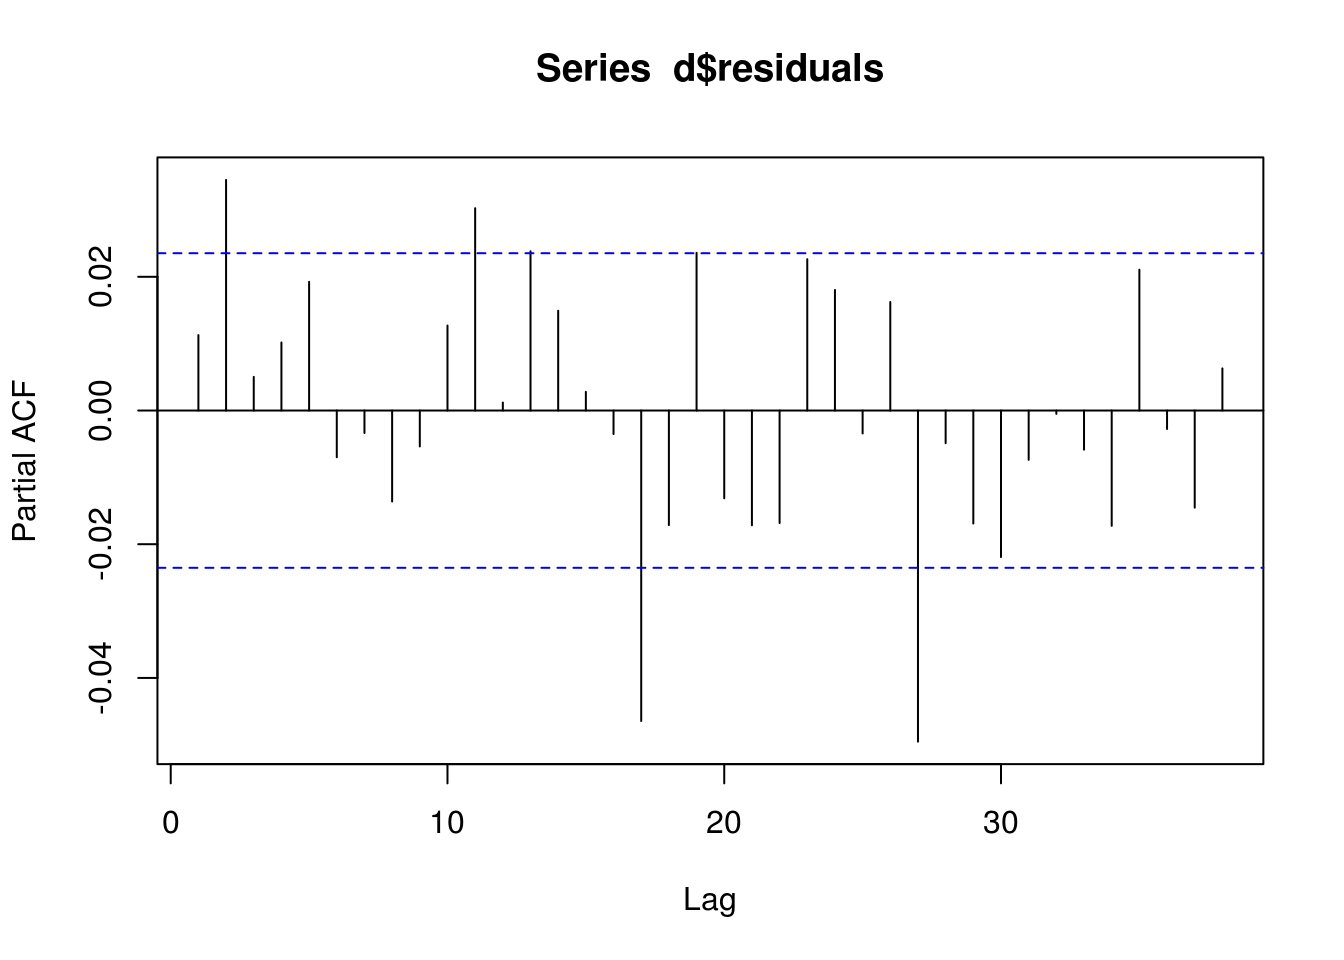
\includegraphics{website_files/figure-latex/unnamed-chunk-16-1.pdf}

Here we see that our parametric seasonality model has accounted for all
of the associations in the data, so there is no autocorrelation in the
residuals:

\begin{Shaded}
\begin{Highlighting}[]
\NormalTok{d[, residuals }\OperatorTok{:}\ErrorTok{=}\StringTok{ }\KeywordTok{residuals}\NormalTok{(pfit1, }\DataTypeTok{type =} \StringTok{"response"}\NormalTok{)]}
\NormalTok{d[, predicted }\OperatorTok{:}\ErrorTok{=}\StringTok{ }\KeywordTok{predict}\NormalTok{(pfit1, }\DataTypeTok{type =} \StringTok{"response"}\NormalTok{)]}
\KeywordTok{pacf}\NormalTok{(d}\OperatorTok{$}\NormalTok{residuals)}
\end{Highlighting}
\end{Shaded}

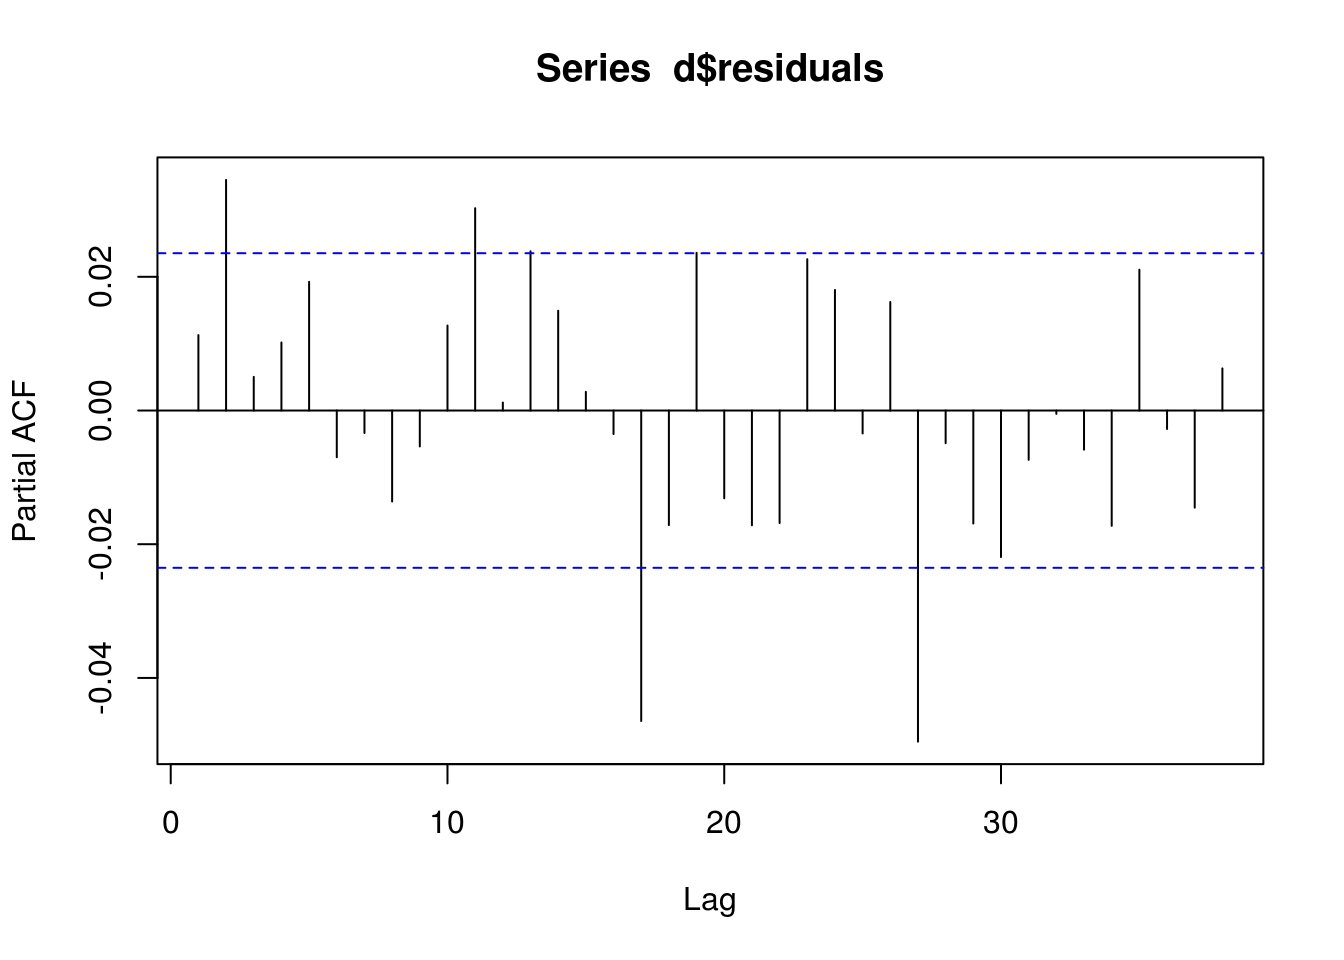
\includegraphics{website_files/figure-latex/unnamed-chunk-17-1.pdf}

\section{Hints For Future Analyses}\label{hints-for-future-analyses}

\subsection{Always Use A Denominator}\label{always-use-a-denominator}

\begin{Shaded}
\begin{Highlighting}[]
\NormalTok{d <-}\StringTok{ }\KeywordTok{data.table}\NormalTok{(}
  \DataTypeTok{year =} \KeywordTok{c}\NormalTok{(}\StringTok{"1950"}\NormalTok{, }\StringTok{"2018"}\NormalTok{),}
  \DataTypeTok{Cases =} \KeywordTok{c}\NormalTok{(}\DecValTok{350000}\NormalTok{, }\DecValTok{530000}\NormalTok{),}
  \DataTypeTok{Population =} \KeywordTok{c}\NormalTok{(}\DecValTok{3500000}\NormalTok{, }\DecValTok{5300000}\NormalTok{)}
\NormalTok{)}
\NormalTok{d[, }\StringTok{`}\DataTypeTok{Cases per}\CharTok{\textbackslash{}n}\DataTypeTok{100.000 Pop}\StringTok{`} \OperatorTok{:}\ErrorTok{=}\StringTok{ }\NormalTok{Cases }\OperatorTok{/}\StringTok{ }\NormalTok{Population }\OperatorTok{*}\StringTok{ }\DecValTok{100000}\NormalTok{]}
\NormalTok{d <-}\StringTok{ }\KeywordTok{melt.data.table}\NormalTok{(d, }\DataTypeTok{id.vars =} \StringTok{"year"}\NormalTok{)}
\end{Highlighting}
\end{Shaded}

We start out by considering the number of cases of a disease in 1950 and
2018. We see that the number of cases has increased dramatically over
this time period!

\begin{Shaded}
\begin{Highlighting}[]
\NormalTok{q <-}\StringTok{ }\KeywordTok{ggplot}\NormalTok{(d[variable }\OperatorTok{==}\StringTok{ "Cases"}\NormalTok{], }\KeywordTok{aes}\NormalTok{(}\DataTypeTok{x =}\NormalTok{ year, }\DataTypeTok{y =}\NormalTok{ value, }\DataTypeTok{fill =}\NormalTok{ variable))}
\NormalTok{q <-}\StringTok{ }\NormalTok{q }\OperatorTok{+}\StringTok{ }\KeywordTok{geom_col}\NormalTok{()}
\NormalTok{q <-}\StringTok{ }\NormalTok{q }\OperatorTok{+}\StringTok{ }\KeywordTok{scale_x_discrete}\NormalTok{(}\StringTok{"Year"}\NormalTok{)}
\NormalTok{q <-}\StringTok{ }\NormalTok{q }\OperatorTok{+}\StringTok{ }\KeywordTok{scale_y_continuous}\NormalTok{(}\StringTok{"Number of people"}\NormalTok{, }\DataTypeTok{labels =}\NormalTok{ scales}\OperatorTok{::}\KeywordTok{format_format}\NormalTok{(}
  \DataTypeTok{big.mark =} \StringTok{"."}\NormalTok{,}
  \DataTypeTok{decimal.mark =} \StringTok{","}\NormalTok{,}
  \DataTypeTok{scientific =} \OtherTok{FALSE}
\NormalTok{))}
\NormalTok{q <-}\StringTok{ }\NormalTok{q }\OperatorTok{+}\StringTok{ }\KeywordTok{scale_fill_brewer}\NormalTok{(}\StringTok{""}\NormalTok{, }\DataTypeTok{palette =} \StringTok{"Set1"}\NormalTok{)}
\NormalTok{q}
\end{Highlighting}
\end{Shaded}

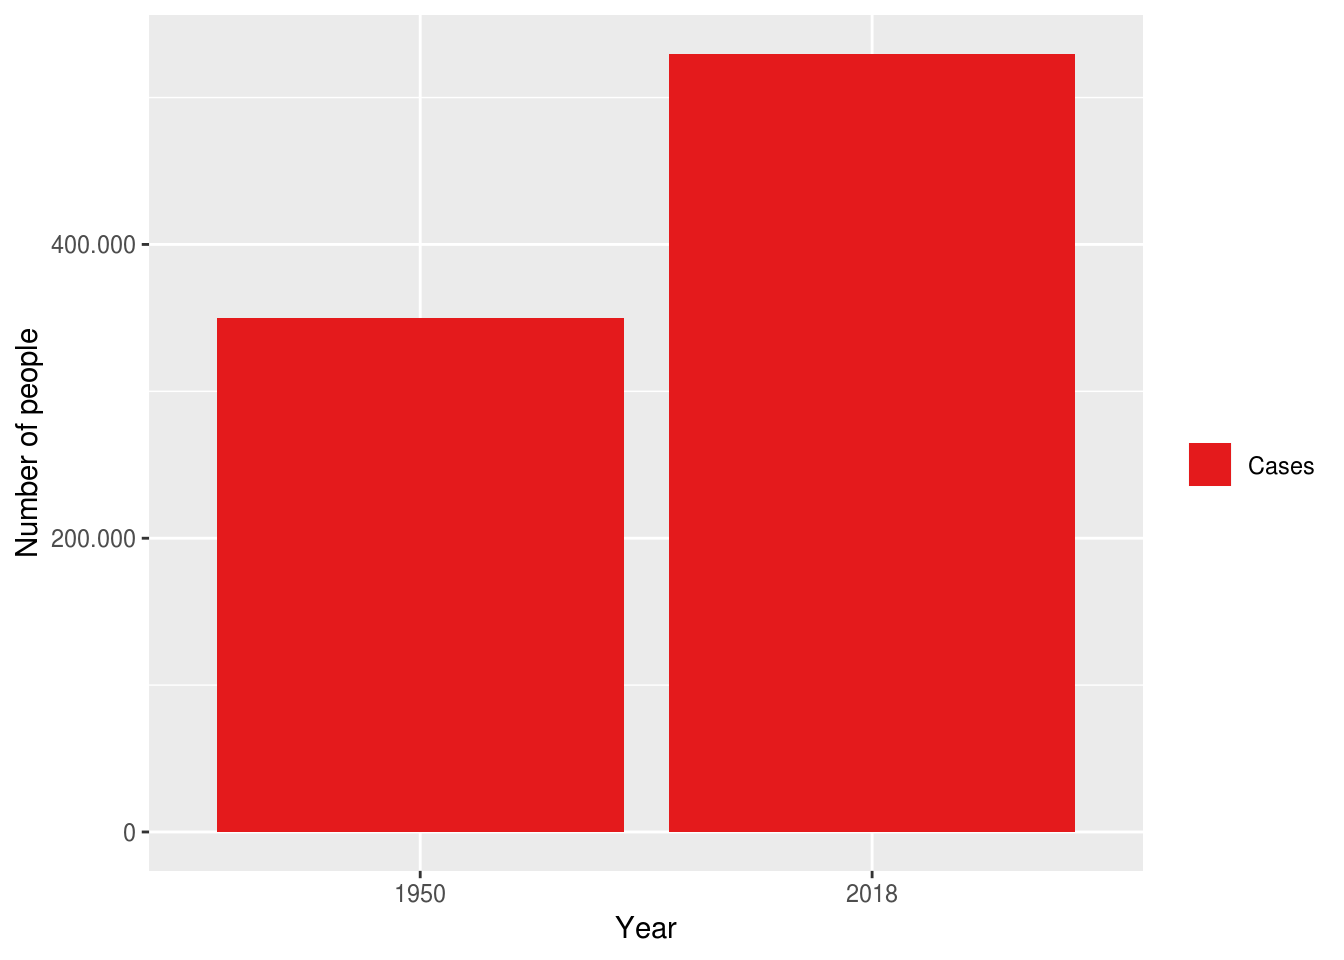
\includegraphics{website_files/figure-latex/unnamed-chunk-19-1.pdf}

However, upon taking the denominator (i.e.~population) into
consideration, we can see that the rate is consistent over time.

\begin{Shaded}
\begin{Highlighting}[]
\NormalTok{q <-}\StringTok{ }\KeywordTok{ggplot}\NormalTok{(d, }\KeywordTok{aes}\NormalTok{(}\DataTypeTok{x =}\NormalTok{ year, }\DataTypeTok{y =}\NormalTok{ value, }\DataTypeTok{fill =}\NormalTok{ variable))}
\NormalTok{q <-}\StringTok{ }\NormalTok{q }\OperatorTok{+}\StringTok{ }\KeywordTok{geom_col}\NormalTok{(}\DataTypeTok{position =} \StringTok{"dodge"}\NormalTok{)}
\NormalTok{q <-}\StringTok{ }\NormalTok{q }\OperatorTok{+}\StringTok{ }\KeywordTok{scale_x_discrete}\NormalTok{(}\StringTok{""}\NormalTok{)}
\NormalTok{q <-}\StringTok{ }\NormalTok{q }\OperatorTok{+}\StringTok{ }\KeywordTok{scale_y_continuous}\NormalTok{(}\StringTok{""}\NormalTok{, }\DataTypeTok{labels =}\NormalTok{ scales}\OperatorTok{::}\KeywordTok{format_format}\NormalTok{(}
  \DataTypeTok{big.mark =} \StringTok{"."}\NormalTok{,}
  \DataTypeTok{decimal.mark =} \StringTok{","}\NormalTok{,}
  \DataTypeTok{scientific =} \OtherTok{FALSE}
\NormalTok{))}
\NormalTok{q <-}\StringTok{ }\NormalTok{q }\OperatorTok{+}\StringTok{ }\KeywordTok{scale_fill_brewer}\NormalTok{(}\StringTok{""}\NormalTok{, }\DataTypeTok{palette =} \StringTok{"Set1"}\NormalTok{)}
\NormalTok{q <-}\StringTok{ }\NormalTok{q }\OperatorTok{+}\StringTok{ }\KeywordTok{facet_wrap}\NormalTok{(}\OperatorTok{~}\NormalTok{variable, }\DataTypeTok{scales =} \StringTok{"free"}\NormalTok{)}
\NormalTok{q}
\end{Highlighting}
\end{Shaded}

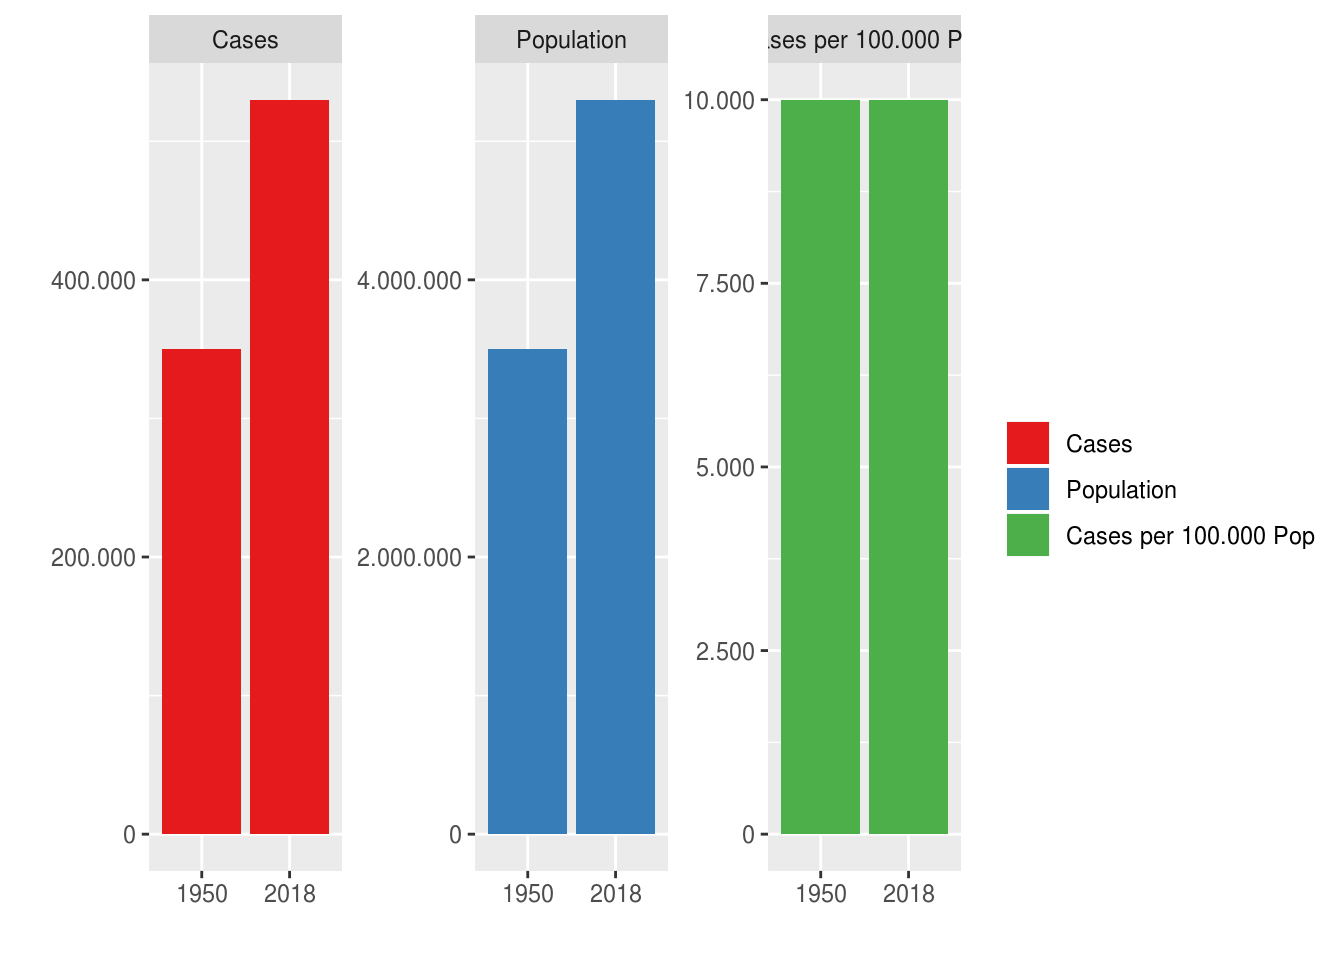
\includegraphics{website_files/figure-latex/unnamed-chunk-20-1.pdf}

\subsection{Negative Binomial Is Generally Better Than
Poisson}\label{negative-binomial-is-generally-better-than-poisson}

Let us consider linear regression.

A linear regression model takes the form:

\[
y_i = \beta_0 + \beta_1 \times x_i + \text{error}_i
\]

Where

\[
\text{error}_i \sim N(0, \sigma)
\] So basically, we have a straight line, and then the data is expected
to be in a parallel band surrounding it:

\begin{Shaded}
\begin{Highlighting}[]
\NormalTok{d <-}\StringTok{ }\KeywordTok{data.table}\NormalTok{(}\DataTypeTok{x =} \KeywordTok{runif}\NormalTok{(}\DecValTok{1000}\NormalTok{) }\OperatorTok{*}\StringTok{ }\DecValTok{10}\NormalTok{)}
\NormalTok{d[, y }\OperatorTok{:}\ErrorTok{=}\StringTok{ }\DecValTok{3} \OperatorTok{+}\StringTok{ }\DecValTok{2} \OperatorTok{*}\StringTok{ }\NormalTok{x }\OperatorTok{+}\StringTok{ }\KeywordTok{rnorm}\NormalTok{(.N)]}

\NormalTok{fit <-}\StringTok{ }\KeywordTok{lm}\NormalTok{(y }\OperatorTok{~}\StringTok{ }\NormalTok{x, }\DataTypeTok{data =}\NormalTok{ d)}
\NormalTok{resid_sd <-}\StringTok{ }\KeywordTok{sd}\NormalTok{(fit}\OperatorTok{$}\NormalTok{residuals)}

\NormalTok{thresholds <-}\StringTok{ }\KeywordTok{data.table}\NormalTok{(}\DataTypeTok{x =} \KeywordTok{c}\NormalTok{(}\DecValTok{0}\OperatorTok{:}\DecValTok{10}\NormalTok{))}
\NormalTok{thresholds[, pred }\OperatorTok{:}\ErrorTok{=}\StringTok{ }\KeywordTok{predict}\NormalTok{(fit, }\DataTypeTok{newdata =}\NormalTok{ thresholds)]}
\NormalTok{thresholds[, pred_l95 }\OperatorTok{:}\ErrorTok{=}\StringTok{ }\NormalTok{pred }\OperatorTok{-}\StringTok{ }\FloatTok{1.96} \OperatorTok{*}\StringTok{ }\NormalTok{resid_sd]}
\NormalTok{thresholds[, pred_u95 }\OperatorTok{:}\ErrorTok{=}\StringTok{ }\NormalTok{pred }\OperatorTok{+}\StringTok{ }\FloatTok{1.96} \OperatorTok{*}\StringTok{ }\NormalTok{resid_sd]}

\NormalTok{q <-}\StringTok{ }\KeywordTok{ggplot}\NormalTok{(d, }\KeywordTok{aes}\NormalTok{(}\DataTypeTok{x =}\NormalTok{ x))}
\NormalTok{q <-}\StringTok{ }\NormalTok{q }\OperatorTok{+}\StringTok{ }\KeywordTok{geom_point}\NormalTok{(}\DataTypeTok{mapping =} \KeywordTok{aes}\NormalTok{(}\DataTypeTok{y =}\NormalTok{ y))}
\NormalTok{q <-}\StringTok{ }\NormalTok{q }\OperatorTok{+}\StringTok{ }\KeywordTok{geom_ribbon}\NormalTok{(}\DataTypeTok{data =}\NormalTok{ thresholds, }\DataTypeTok{mapping =} \KeywordTok{aes}\NormalTok{(}\DataTypeTok{ymin =}\NormalTok{ pred_l95, }\DataTypeTok{ymax =}\NormalTok{ pred_u95), }\DataTypeTok{alpha =} \FloatTok{0.5}\NormalTok{)}
\NormalTok{q <-}\StringTok{ }\NormalTok{q }\OperatorTok{+}\StringTok{ }\KeywordTok{geom_line}\NormalTok{(}\DataTypeTok{data =}\NormalTok{ thresholds, }\DataTypeTok{mapping =} \KeywordTok{aes}\NormalTok{(}\DataTypeTok{y =}\NormalTok{ pred), }\DataTypeTok{colour =} \StringTok{"red"}\NormalTok{, }\DataTypeTok{lwd =} \DecValTok{2}\NormalTok{)}
\NormalTok{q}
\end{Highlighting}
\end{Shaded}

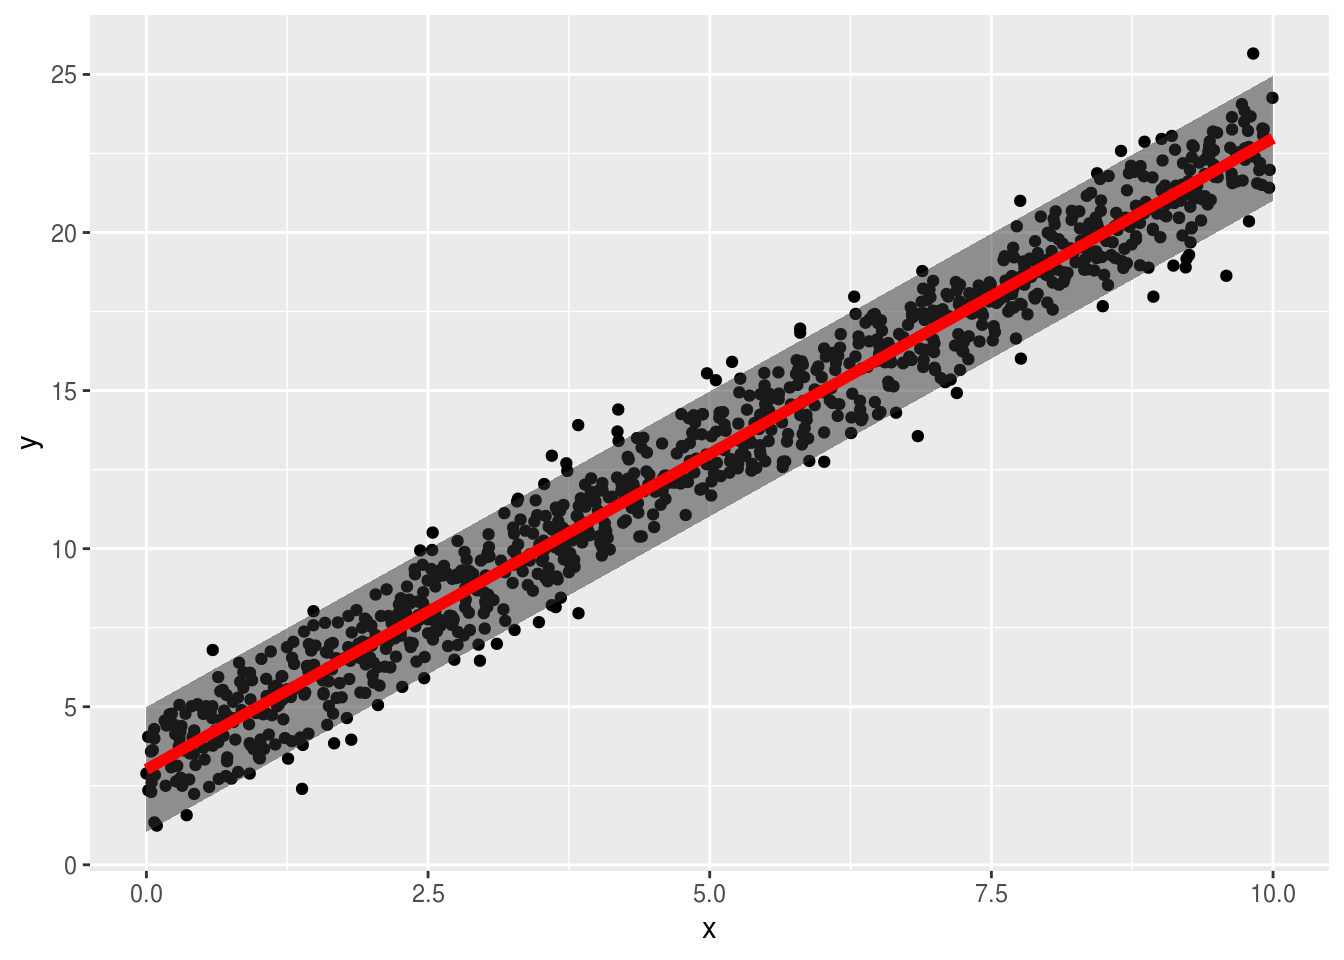
\includegraphics{website_files/figure-latex/unnamed-chunk-21-1.pdf}

Poisson regression operates under the strong assumption that
\texttt{mean=variance}. This means that when the mean is 150 (e.g.~150
cases per day), then the variance is also 150 (e.g.~we expect between
126 and 174 cases each day). When the mean is 5 (e.g.~5 cases per day),
then the variance is also 5 (e.g.~we expect between 1 and 10 cases each
day).

\begin{Shaded}
\begin{Highlighting}[]
\NormalTok{d <-}\StringTok{ }\KeywordTok{data.table}\NormalTok{(}\DataTypeTok{x =} \KeywordTok{runif}\NormalTok{(}\DecValTok{1000}\NormalTok{) }\OperatorTok{*}\StringTok{ }\DecValTok{5}\NormalTok{)}
\NormalTok{d[, mu }\OperatorTok{:}\ErrorTok{=}\StringTok{ }\KeywordTok{exp}\NormalTok{(}\FloatTok{0.1} \OperatorTok{+}\StringTok{ }\NormalTok{x)]}
\NormalTok{d[, y }\OperatorTok{:}\ErrorTok{=}\StringTok{ }\KeywordTok{rpois}\NormalTok{(.N, mu)]}

\NormalTok{fit <-}\StringTok{ }\KeywordTok{glm}\NormalTok{(y }\OperatorTok{~}\StringTok{ }\NormalTok{x, }\DataTypeTok{data =}\NormalTok{ d, }\DataTypeTok{family =} \StringTok{"poisson"}\NormalTok{)}
\NormalTok{resid_sd <-}\StringTok{ }\KeywordTok{sd}\NormalTok{(fit}\OperatorTok{$}\NormalTok{residuals)}

\NormalTok{thresholds <-}\StringTok{ }\KeywordTok{data.table}\NormalTok{(}\DataTypeTok{x =} \KeywordTok{c}\NormalTok{(}\DecValTok{0}\OperatorTok{:}\DecValTok{50}\NormalTok{) }\OperatorTok{/}\StringTok{ }\DecValTok{10}\NormalTok{)}
\NormalTok{thresholds[, pred }\OperatorTok{:}\ErrorTok{=}\StringTok{ }\KeywordTok{predict}\NormalTok{(fit, }\DataTypeTok{newdata =}\NormalTok{ thresholds, }\DataTypeTok{type =} \StringTok{"response"}\NormalTok{)]}
\NormalTok{thresholds[, pred_l95 }\OperatorTok{:}\ErrorTok{=}\StringTok{ }\KeywordTok{qpois}\NormalTok{(}\FloatTok{0.025}\NormalTok{, pred)]}
\NormalTok{thresholds[, pred_u95 }\OperatorTok{:}\ErrorTok{=}\StringTok{ }\KeywordTok{qpois}\NormalTok{(}\FloatTok{0.975}\NormalTok{, pred)]}

\NormalTok{q <-}\StringTok{ }\KeywordTok{ggplot}\NormalTok{(d, }\KeywordTok{aes}\NormalTok{(}\DataTypeTok{x =}\NormalTok{ x))}
\NormalTok{q <-}\StringTok{ }\NormalTok{q }\OperatorTok{+}\StringTok{ }\KeywordTok{geom_point}\NormalTok{(}\DataTypeTok{mapping =} \KeywordTok{aes}\NormalTok{(}\DataTypeTok{y =}\NormalTok{ y))}
\NormalTok{q <-}\StringTok{ }\NormalTok{q }\OperatorTok{+}\StringTok{ }\KeywordTok{geom_ribbon}\NormalTok{(}\DataTypeTok{data =}\NormalTok{ thresholds, }\DataTypeTok{mapping =} \KeywordTok{aes}\NormalTok{(}\DataTypeTok{ymin =}\NormalTok{ pred_l95, }\DataTypeTok{ymax =}\NormalTok{ pred_u95), }\DataTypeTok{alpha =} \FloatTok{0.5}\NormalTok{)}
\NormalTok{q <-}\StringTok{ }\NormalTok{q }\OperatorTok{+}\StringTok{ }\KeywordTok{geom_line}\NormalTok{(}\DataTypeTok{data =}\NormalTok{ thresholds, }\DataTypeTok{mapping =} \KeywordTok{aes}\NormalTok{(}\DataTypeTok{y =}\NormalTok{ pred), }\DataTypeTok{colour =} \StringTok{"red"}\NormalTok{, }\DataTypeTok{lwd =} \DecValTok{2}\NormalTok{)}
\NormalTok{q}
\end{Highlighting}
\end{Shaded}

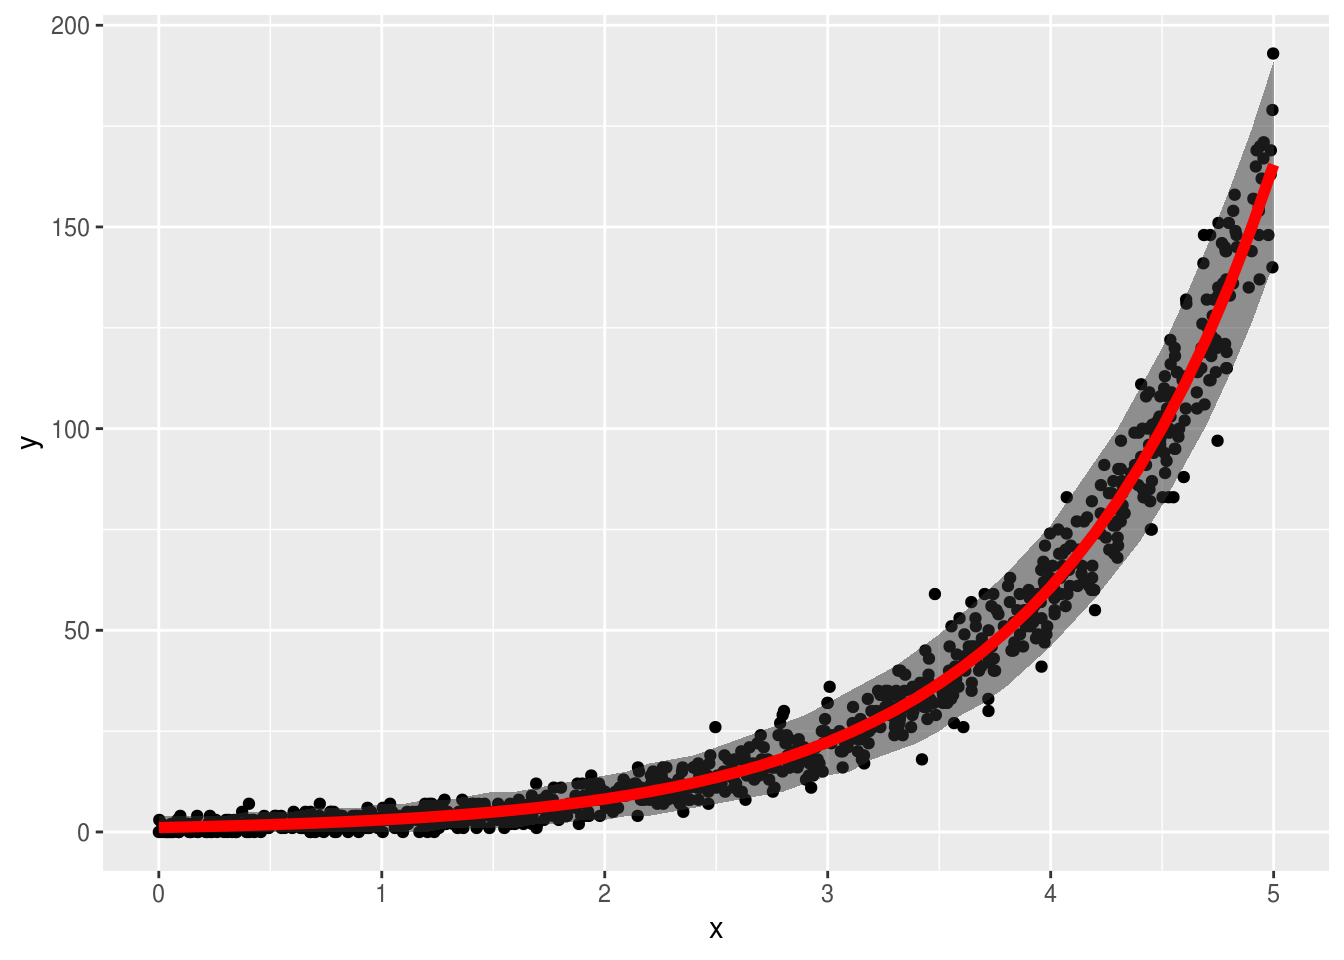
\includegraphics{website_files/figure-latex/unnamed-chunk-22-1.pdf}

This assumption may be true, or it may not be true. However, the main
point is that it is a strong assumption, which makes the poisson
regression less flexible.

A more flexible regression model for count data is the negative binomial
model. Here, the ``dispersion'' (i.e.~variance of the data) is estimated
separately from the mean. You can think of it as being similar to a
linear regression.

The benefits of the negative binomial regression model is that it is
more flexible and is more likely to fit your data.

The downside of the negative binomial regression model is that it needs
more data and may not converge. It is recommended to try and run a
negative binomial regression model first, and then if it fails to
converge, then run a poisson regression.

\subsection{Zeroes In Your Individial -\textgreater{} Aggregated
Dataset}\label{zeroes-in-your-individial---aggregated-dataset}

If your data is at the individual level (i.e.~one row per case), then
you will need to aggregate it to daily/weekly/monthly levels. If your
data source is a registry, and you assume that your dataset contains all
of the reported cases, then this means
\texttt{"no\ reports"="no\ cases"}. This means that after aggregating,
\textbf{you need to make sure that your collapsed/aggregated dataset has
zeroes in it!!}

In the following dataset, we have one case per day from
\texttt{2000-01-01} until \texttt{2000-01-29} and then again one case
per day from \texttt{2000-08-08} until \texttt{2000-12-31}.

\begin{Shaded}
\begin{Highlighting}[]
\NormalTok{d <-}\StringTok{ }\KeywordTok{data.table}\NormalTok{(}\DataTypeTok{date =} \KeywordTok{seq.Date}\NormalTok{(}
  \DataTypeTok{from =} \KeywordTok{as.Date}\NormalTok{(}\StringTok{"2000-01-01"}\NormalTok{),}
  \DataTypeTok{to =} \KeywordTok{as.Date}\NormalTok{(}\StringTok{"2000-12-31"}\NormalTok{),}
  \DataTypeTok{by =} \DecValTok{1}
\NormalTok{))}
\NormalTok{d <-}\StringTok{ }\NormalTok{d[}\OperatorTok{-}\KeywordTok{c}\NormalTok{(}\DecValTok{30}\OperatorTok{:}\DecValTok{220}\NormalTok{)]}
\NormalTok{d[, id }\OperatorTok{:}\ErrorTok{=}\StringTok{ }\DecValTok{1}\OperatorTok{:}\NormalTok{.N]}
\NormalTok{d[, month }\OperatorTok{:}\ErrorTok{=}\StringTok{ }\KeywordTok{as.numeric}\NormalTok{(}\KeywordTok{format.Date}\NormalTok{(date, }\StringTok{"%m"}\NormalTok{))]}

\KeywordTok{print}\NormalTok{(d)}
\end{Highlighting}
\end{Shaded}

\begin{verbatim}
##            date  id month
##   1: 2000-01-01   1     1
##   2: 2000-01-02   2     1
##   3: 2000-01-03   3     1
##   4: 2000-01-04   4     1
##   5: 2000-01-05   5     1
##  ---                     
## 171: 2000-12-27 171    12
## 172: 2000-12-28 172    12
## 173: 2000-12-29 173    12
## 174: 2000-12-30 174    12
## 175: 2000-12-31 175    12
\end{verbatim}

If we collapse the data into months:

\begin{Shaded}
\begin{Highlighting}[]
\NormalTok{collapsed <-}\StringTok{ }\NormalTok{d[, .(}
  \DataTypeTok{n =}\NormalTok{ .N}
\NormalTok{), keyby =}\StringTok{ }\NormalTok{.(}
\NormalTok{  month}
\NormalTok{)]}

\KeywordTok{print}\NormalTok{(collapsed)}
\end{Highlighting}
\end{Shaded}

\begin{verbatim}
##    month  n
## 1:     1 29
## 2:     8 24
## 3:     9 30
## 4:    10 31
## 5:    11 30
## 6:    12 31
\end{verbatim}

You see that we are missing months \texttt{1} through to \texttt{6}. We
cannot analyse this data, because \textbf{we do not have any zeros}.

How do we fix this? We create a \texttt{skeleton} of our results:

\begin{Shaded}
\begin{Highlighting}[]
\NormalTok{skeleton <-}\StringTok{ }\KeywordTok{data.table}\NormalTok{(}\DataTypeTok{month =} \DecValTok{1}\OperatorTok{:}\DecValTok{12}\NormalTok{)}
\KeywordTok{print}\NormalTok{(skeleton)}
\end{Highlighting}
\end{Shaded}

\begin{verbatim}
##     month
##  1:     1
##  2:     2
##  3:     3
##  4:     4
##  5:     5
##  6:     6
##  7:     7
##  8:     8
##  9:     9
## 10:    10
## 11:    11
## 12:    12
\end{verbatim}

We then merge our collapsed data with the skeleton:

\begin{Shaded}
\begin{Highlighting}[]
\NormalTok{final <-}\StringTok{ }\KeywordTok{merge}\NormalTok{(skeleton, collapsed, }\DataTypeTok{by =} \StringTok{"month"}\NormalTok{, }\DataTypeTok{all.x =} \OtherTok{TRUE}\NormalTok{)}
\KeywordTok{print}\NormalTok{(final)}
\end{Highlighting}
\end{Shaded}

\begin{verbatim}
##     month  n
##  1:     1 29
##  2:     2 NA
##  3:     3 NA
##  4:     4 NA
##  5:     5 NA
##  6:     6 NA
##  7:     7 NA
##  8:     8 24
##  9:     9 30
## 10:    10 31
## 11:    11 30
## 12:    12 31
\end{verbatim}

We then set all of the ``missing'' to 0:

\begin{Shaded}
\begin{Highlighting}[]
\NormalTok{final[}\KeywordTok{is.na}\NormalTok{(n), n }\OperatorTok{:}\ErrorTok{=}\StringTok{ }\DecValTok{0}\NormalTok{]}
\KeywordTok{print}\NormalTok{(final)}
\end{Highlighting}
\end{Shaded}

\begin{verbatim}
##     month  n
##  1:     1 29
##  2:     2  0
##  3:     3  0
##  4:     4  0
##  5:     5  0
##  6:     6  0
##  7:     7  0
##  8:     8 24
##  9:     9 30
## 10:    10 31
## 11:    11 30
## 12:    12 31
\end{verbatim}

Now we can analyze our data!

\subsection{Lagging Of Exposures}\label{lagging-of-exposures}

If you are interested in seeing how exposures affect your outcome (e.g.
\texttt{rainfall}) then you might want to consider lagging your
exposure. This will show you
\texttt{how\ did\ the\ rainfall\ from\ last\ week\ affect\ the\ number\ of\ cases\ this\ week?}

\chapter{Panel data - Multiple Areas}\label{panel-data---multiple-areas}

\section{Aim}\label{aim-1}

We are given a dataset containing yearly counts of diseases from
multiple geographical areas.

We will explore how this is different from the one area case.

For this section, we will use linear regression to make the calculations
easier to work with, but the principle is the same as with poisson and
negative binomial regression.

\section{Creating the data}\label{creating-the-data}

\begin{Shaded}
\begin{Highlighting}[]
\KeywordTok{library}\NormalTok{(data.table)}
\KeywordTok{library}\NormalTok{(lme4)}
\end{Highlighting}
\end{Shaded}

\begin{verbatim}
## Loading required package: Matrix
\end{verbatim}

\begin{Shaded}
\begin{Highlighting}[]
\KeywordTok{library}\NormalTok{(ggplot2)}
\KeywordTok{set.seed}\NormalTok{(}\DecValTok{4}\NormalTok{)}

\NormalTok{fylkeIntercepts <-}\StringTok{ }\KeywordTok{data.table}\NormalTok{(}\DataTypeTok{fylke =} \DecValTok{1}\OperatorTok{:}\DecValTok{3}\NormalTok{, }\DataTypeTok{fylkeIntercepts =} \KeywordTok{c}\NormalTok{(}\DecValTok{30}\NormalTok{, }\DecValTok{0}\NormalTok{, }\OperatorTok{-}\DecValTok{30}\NormalTok{))}

\NormalTok{d <-}\StringTok{ }\KeywordTok{data.table}\NormalTok{(}\DataTypeTok{fylke =} \KeywordTok{rep}\NormalTok{(}\DecValTok{1}\OperatorTok{:}\DecValTok{3}\NormalTok{, }\DataTypeTok{each =} \DecValTok{100}\NormalTok{))}
\NormalTok{d <-}\StringTok{ }\KeywordTok{merge}\NormalTok{(d, fylkeIntercepts, }\DataTypeTok{by =} \StringTok{"fylke"}\NormalTok{)}
\NormalTok{d[, mainIntercept }\OperatorTok{:}\ErrorTok{=}\StringTok{ }\DecValTok{5}\NormalTok{]}
\NormalTok{d[, x }\OperatorTok{:}\ErrorTok{=}\StringTok{ }\KeywordTok{runif}\NormalTok{(.N)]}
\NormalTok{d[, year }\OperatorTok{:}\ErrorTok{=}\StringTok{ }\KeywordTok{sample}\NormalTok{(}\KeywordTok{c}\NormalTok{(}\DecValTok{1950}\OperatorTok{:}\DecValTok{2020}\NormalTok{), .N, }\DataTypeTok{replace =}\NormalTok{ T)]}
\NormalTok{d[, yearMinus1950 }\OperatorTok{:}\ErrorTok{=}\StringTok{ }\NormalTok{year }\OperatorTok{-}\StringTok{ }\DecValTok{1950}\NormalTok{]}
\NormalTok{d[, mu }\OperatorTok{:}\ErrorTok{=}\StringTok{ }\NormalTok{mainIntercept }\OperatorTok{+}\StringTok{ }\NormalTok{fylkeIntercepts }\OperatorTok{+}\StringTok{ }\FloatTok{0.5} \OperatorTok{*}\StringTok{ }\NormalTok{yearMinus1950]}
\NormalTok{d[, y }\OperatorTok{:}\ErrorTok{=}\StringTok{ }\KeywordTok{round}\NormalTok{(}\KeywordTok{rnorm}\NormalTok{(.N, mu, }\DataTypeTok{sd =} \DecValTok{1}\NormalTok{))]}
\CommentTok{# d[,y:=rpois(.N,mu)]}

\NormalTok{d[fylke }\OperatorTok{==}\StringTok{ }\DecValTok{1} \OperatorTok{&}\StringTok{ }\OperatorTok{!}\NormalTok{year }\OperatorTok\StringTok{ }\KeywordTok{c}\NormalTok{(}\DecValTok{1950}\OperatorTok{:}\DecValTok{1980}\NormalTok{), y }\OperatorTok{:}\ErrorTok{=}\StringTok{ }\OtherTok{NA}\NormalTok{]}
\NormalTok{d[fylke }\OperatorTok{==}\StringTok{ }\DecValTok{2} \OperatorTok{&}\StringTok{ }\OperatorTok{!}\NormalTok{year }\OperatorTok\StringTok{ }\KeywordTok{c}\NormalTok{(}\DecValTok{1980}\OperatorTok{:}\DecValTok{2000}\NormalTok{), y }\OperatorTok{:}\ErrorTok{=}\StringTok{ }\OtherTok{NA}\NormalTok{]}
\NormalTok{d[fylke }\OperatorTok{==}\StringTok{ }\DecValTok{3} \OperatorTok{&}\StringTok{ }\OperatorTok{!}\NormalTok{year }\OperatorTok\StringTok{ }\KeywordTok{c}\NormalTok{(}\DecValTok{2000}\OperatorTok{:}\DecValTok{2020}\NormalTok{), y }\OperatorTok{:}\ErrorTok{=}\StringTok{ }\OtherTok{NA}\NormalTok{]}

\NormalTok{d <-}\StringTok{ }\KeywordTok{na.omit}\NormalTok{(d)}
\end{Highlighting}
\end{Shaded}

\newpage

\section{Investigating the data}\label{investigating-the-data}

We begin by blindly looking at the data.

\begin{Shaded}
\begin{Highlighting}[]
\NormalTok{q <-}\StringTok{ }\KeywordTok{ggplot}\NormalTok{(d, }\KeywordTok{aes}\NormalTok{(}\DataTypeTok{x =}\NormalTok{ year, }\DataTypeTok{y =}\NormalTok{ y))}
\NormalTok{q <-}\StringTok{ }\NormalTok{q }\OperatorTok{+}\StringTok{ }\KeywordTok{geom_point}\NormalTok{()}
\NormalTok{q <-}\StringTok{ }\NormalTok{q }\OperatorTok{+}\StringTok{ }\KeywordTok{scale_x_continuous}\NormalTok{(}\StringTok{"Year"}\NormalTok{)}
\NormalTok{q <-}\StringTok{ }\NormalTok{q }\OperatorTok{+}\StringTok{ }\KeywordTok{scale_y_continuous}\NormalTok{(}\StringTok{"Cases"}\NormalTok{)}
\NormalTok{q}
\end{Highlighting}
\end{Shaded}

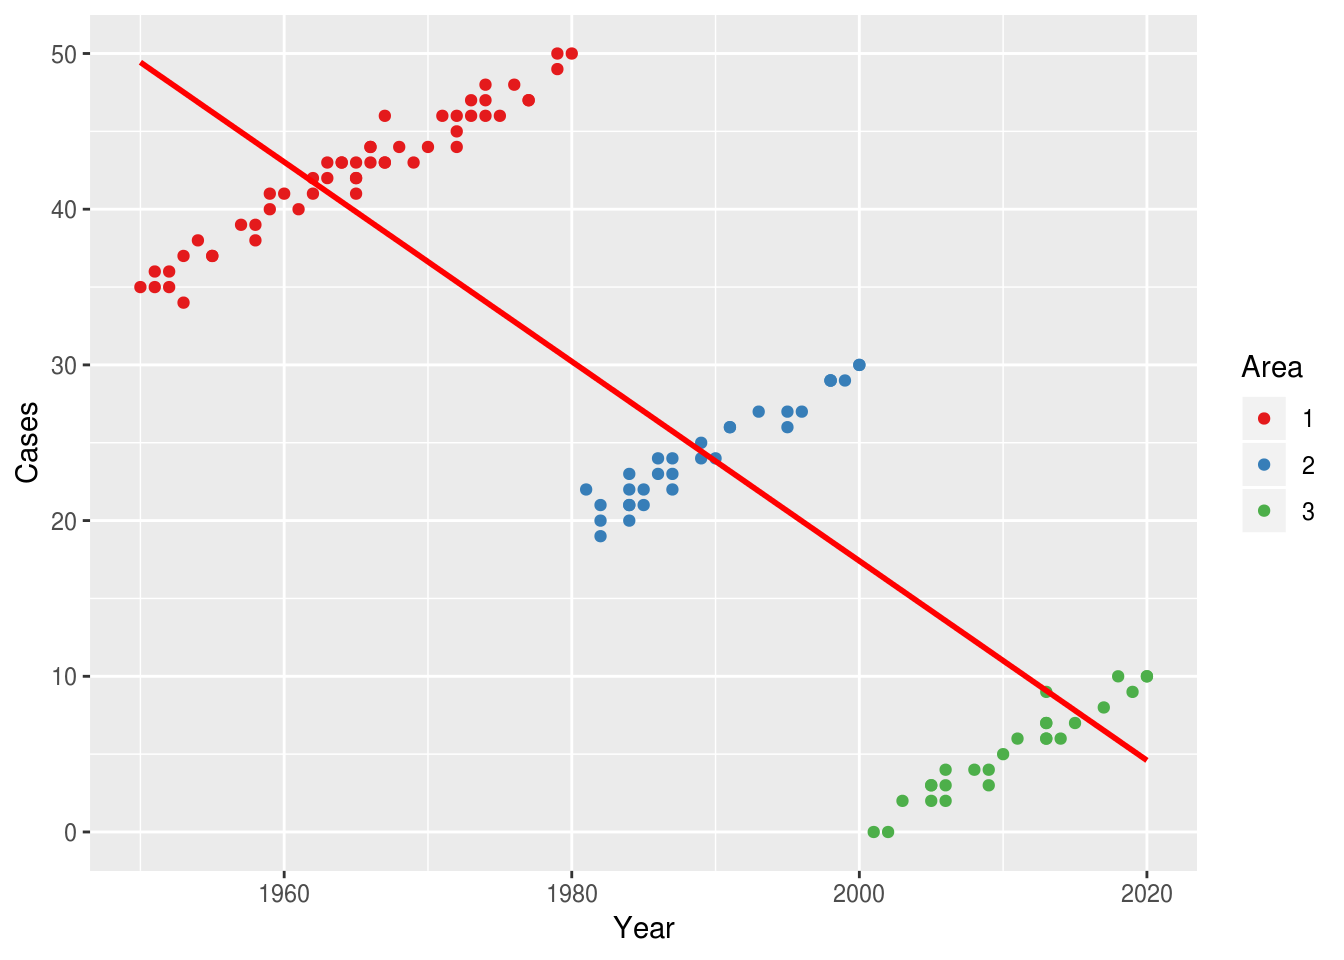
\includegraphics{website_files/figure-latex/unnamed-chunk-29-1.pdf}

We then blindly run a linear regression and we see that the number of
cases is decreasing over time.

\begin{Shaded}
\begin{Highlighting}[]
\NormalTok{q <-}\StringTok{ }\KeywordTok{ggplot}\NormalTok{(d, }\KeywordTok{aes}\NormalTok{(}\DataTypeTok{x =}\NormalTok{ year, }\DataTypeTok{y =}\NormalTok{ y))}
\NormalTok{q <-}\StringTok{ }\NormalTok{q }\OperatorTok{+}\StringTok{ }\KeywordTok{geom_point}\NormalTok{()}
\NormalTok{q <-}\StringTok{ }\NormalTok{q }\OperatorTok{+}\StringTok{ }\KeywordTok{stat_smooth}\NormalTok{(}\DataTypeTok{method =} \StringTok{"lm"}\NormalTok{, }\DataTypeTok{se =}\NormalTok{ F, }\DataTypeTok{colour =} \StringTok{"red"}\NormalTok{)}
\NormalTok{q <-}\StringTok{ }\NormalTok{q }\OperatorTok{+}\StringTok{ }\KeywordTok{scale_x_continuous}\NormalTok{(}\StringTok{"Year"}\NormalTok{)}
\NormalTok{q <-}\StringTok{ }\NormalTok{q }\OperatorTok{+}\StringTok{ }\KeywordTok{scale_y_continuous}\NormalTok{(}\StringTok{"Cases"}\NormalTok{)}
\NormalTok{q}
\end{Highlighting}
\end{Shaded}

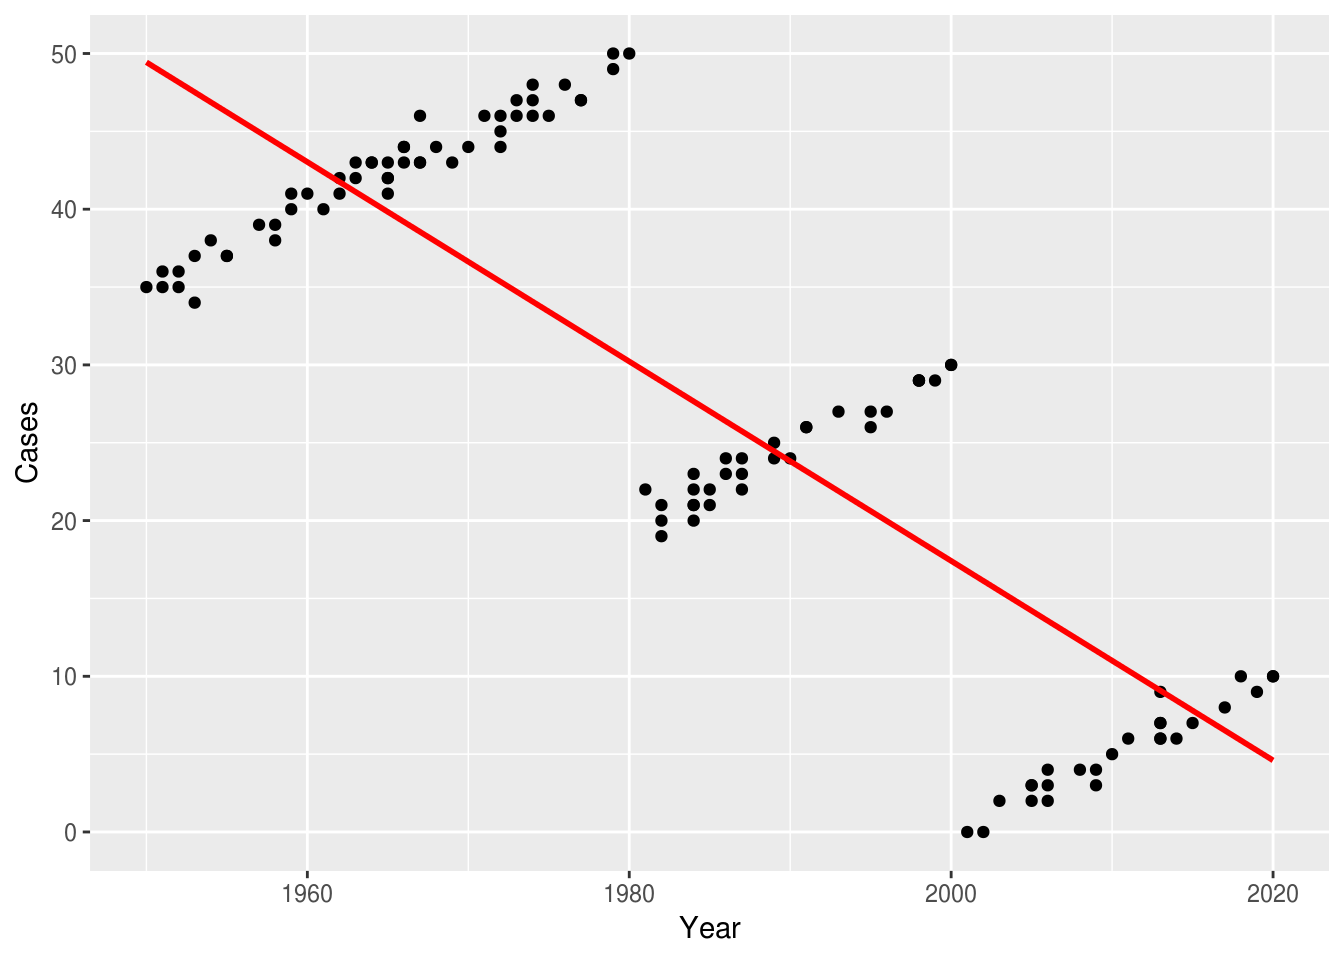
\includegraphics{website_files/figure-latex/unnamed-chunk-30-1.pdf}

However, once we reveal the geographical clustering in the data, we can
see that our regression model is extremely wrong:

\begin{Shaded}
\begin{Highlighting}[]
\NormalTok{q <-}\StringTok{ }\KeywordTok{ggplot}\NormalTok{(d, }\KeywordTok{aes}\NormalTok{(}\DataTypeTok{x =}\NormalTok{ year, }\DataTypeTok{y =}\NormalTok{ y))}
\NormalTok{q <-}\StringTok{ }\NormalTok{q }\OperatorTok{+}\StringTok{ }\KeywordTok{geom_point}\NormalTok{(}\DataTypeTok{mapping =} \KeywordTok{aes}\NormalTok{(}\DataTypeTok{colour =} \KeywordTok{as.factor}\NormalTok{(fylke)))}
\NormalTok{q <-}\StringTok{ }\NormalTok{q }\OperatorTok{+}\StringTok{ }\KeywordTok{stat_smooth}\NormalTok{(}\DataTypeTok{method =} \StringTok{"lm"}\NormalTok{, }\DataTypeTok{se =}\NormalTok{ F, }\DataTypeTok{colour =} \StringTok{"red"}\NormalTok{)}
\NormalTok{q <-}\StringTok{ }\NormalTok{q }\OperatorTok{+}\StringTok{ }\KeywordTok{scale_x_continuous}\NormalTok{(}\StringTok{"Year"}\NormalTok{)}
\NormalTok{q <-}\StringTok{ }\NormalTok{q }\OperatorTok{+}\StringTok{ }\KeywordTok{scale_y_continuous}\NormalTok{(}\StringTok{"Cases"}\NormalTok{)}
\NormalTok{q <-}\StringTok{ }\NormalTok{q }\OperatorTok{+}\StringTok{ }\KeywordTok{scale_colour_brewer}\NormalTok{(}\StringTok{"Area"}\NormalTok{, }\DataTypeTok{palette =} \StringTok{"Set1"}\NormalTok{)}
\NormalTok{q}
\end{Highlighting}
\end{Shaded}

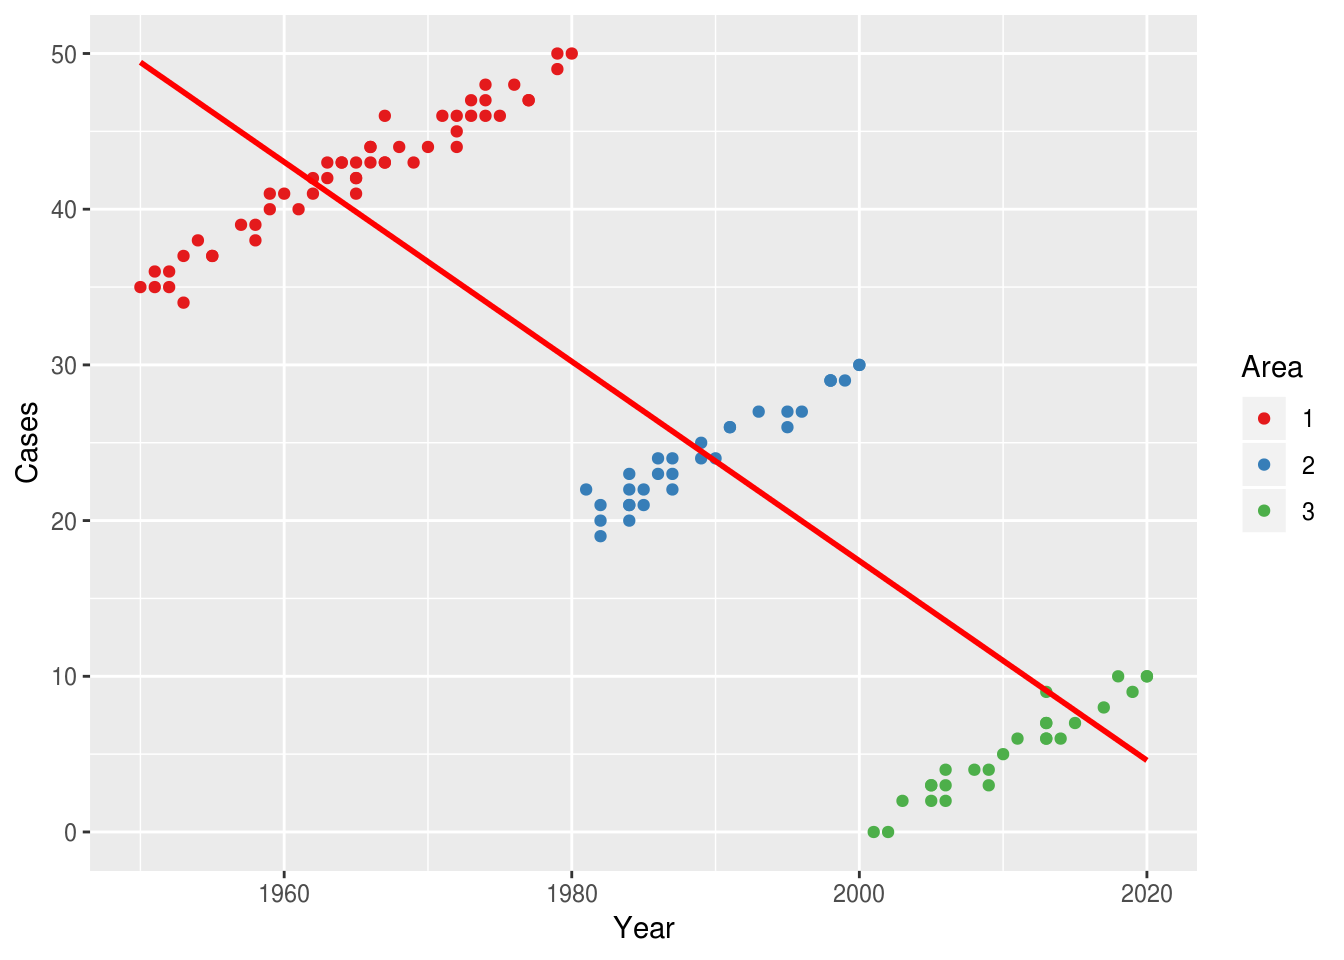
\includegraphics{website_files/figure-latex/unnamed-chunk-31-1.pdf}

\textbf{Note:} The differing \texttt{number\ of\ cases} in each
geographical area could also be due to differing \texttt{populations}.
Always remember to \texttt{use\ a\ denominator}!!!

\section{Time Trend Within Geographical
Areas}\label{time-trend-within-geographical-areas}

What we actually want to do, is observe the time trends \texttt{within}
each geographical area:

\begin{Shaded}
\begin{Highlighting}[]
\NormalTok{fit <-}\StringTok{ }\KeywordTok{lm}\NormalTok{(y }\OperatorTok{~}\StringTok{ }\KeywordTok{as.factor}\NormalTok{(fylke) }\OperatorTok{+}\StringTok{ }\NormalTok{yearMinus1950, }\DataTypeTok{data =}\NormalTok{ d)}
\NormalTok{d[, p }\OperatorTok{:}\ErrorTok{=}\StringTok{ }\KeywordTok{predict}\NormalTok{(fit, }\DataTypeTok{newdata =}\NormalTok{ d)]}

\NormalTok{q <-}\StringTok{ }\KeywordTok{ggplot}\NormalTok{(d, }\KeywordTok{aes}\NormalTok{(}\DataTypeTok{x =}\NormalTok{ year, }\DataTypeTok{y =}\NormalTok{ y))}
\NormalTok{q <-}\StringTok{ }\NormalTok{q }\OperatorTok{+}\StringTok{ }\KeywordTok{geom_point}\NormalTok{(}\DataTypeTok{mapping =} \KeywordTok{aes}\NormalTok{(}\DataTypeTok{colour =} \KeywordTok{as.factor}\NormalTok{(fylke)))}
\NormalTok{q <-}\StringTok{ }\NormalTok{q }\OperatorTok{+}\StringTok{ }\KeywordTok{geom_line}\NormalTok{(}\DataTypeTok{mapping =} \KeywordTok{aes}\NormalTok{(}\DataTypeTok{y =}\NormalTok{ p, }\DataTypeTok{group =} \KeywordTok{as.factor}\NormalTok{(fylke)), }\DataTypeTok{colour =} \StringTok{"red"}\NormalTok{)}
\NormalTok{q <-}\StringTok{ }\NormalTok{q }\OperatorTok{+}\StringTok{ }\KeywordTok{scale_x_continuous}\NormalTok{(}\StringTok{"Year"}\NormalTok{)}
\NormalTok{q <-}\StringTok{ }\NormalTok{q }\OperatorTok{+}\StringTok{ }\KeywordTok{scale_y_continuous}\NormalTok{(}\StringTok{"Cases"}\NormalTok{)}
\NormalTok{q <-}\StringTok{ }\NormalTok{q }\OperatorTok{+}\StringTok{ }\KeywordTok{scale_colour_brewer}\NormalTok{(}\StringTok{"Area"}\NormalTok{, }\DataTypeTok{palette =} \StringTok{"Set1"}\NormalTok{)}
\NormalTok{q}
\end{Highlighting}
\end{Shaded}

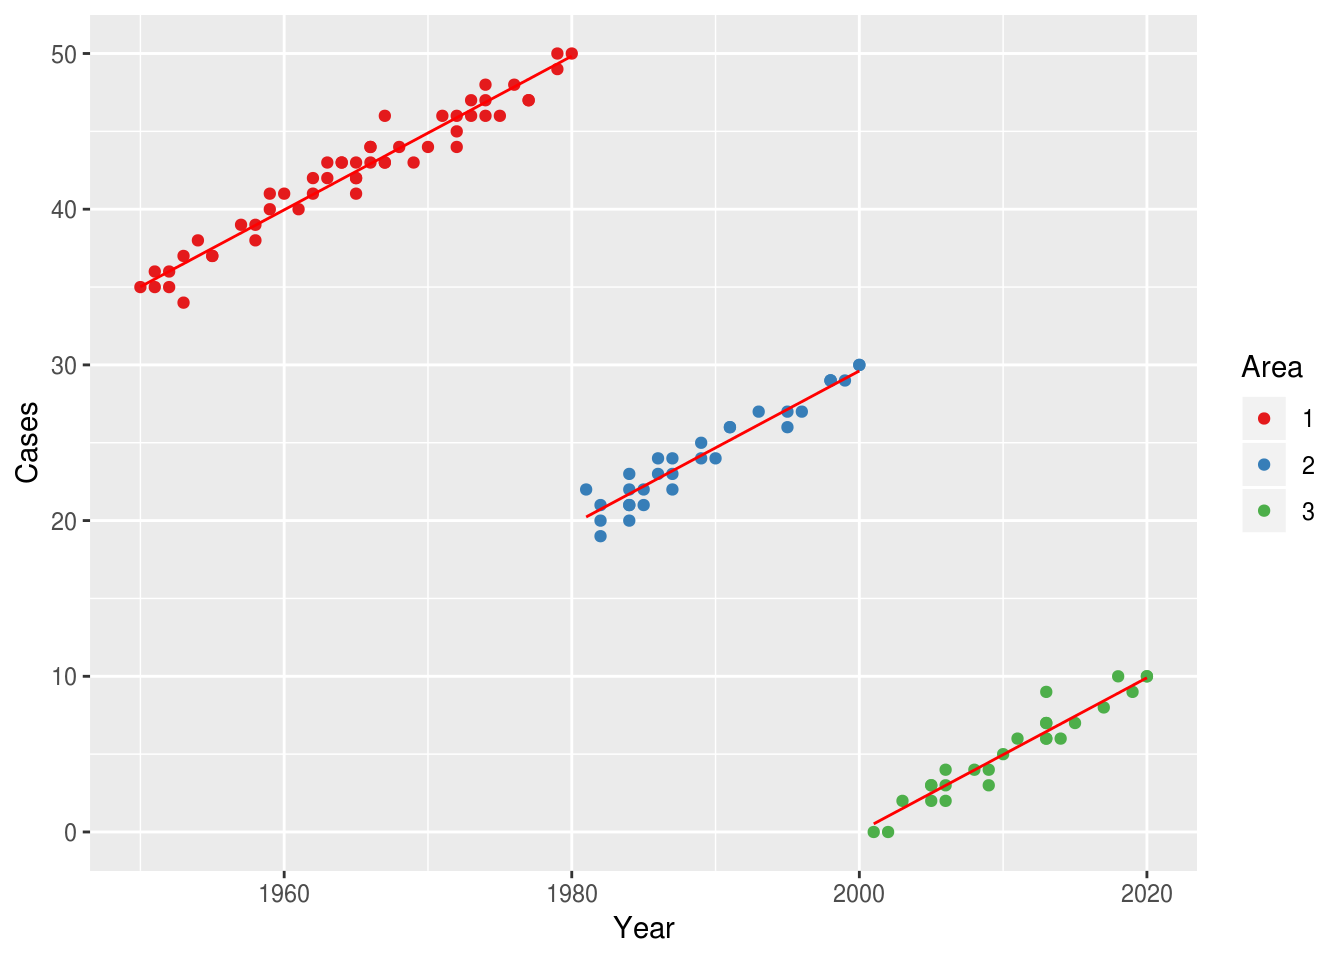
\includegraphics{website_files/figure-latex/unnamed-chunk-32-1.pdf}

So how do we achieve this? Basically, by identifying how the areas
differ from each other, and then raising/lowering each area as
appropriate. The amount that each area differs from the global average
is called the \texttt{area-specific\ intercept}.

Once we have removed the \texttt{area-specific\ intercept} from each
geographical area, we can (basically) just run a normal regression to
find the overall time trend.

\begin{Shaded}
\begin{Highlighting}[]
\NormalTok{d[, yMinusIntercept }\OperatorTok{:}\ErrorTok{=}\StringTok{ }\NormalTok{y]}
\NormalTok{d[fylke }\OperatorTok{==}\StringTok{ }\DecValTok{2}\NormalTok{, yMinusIntercept }\OperatorTok{:}\ErrorTok{=}\StringTok{ }\NormalTok{y }\OperatorTok{-}\StringTok{ }\OperatorTok{-}\FloatTok{30.0944}\NormalTok{]}
\NormalTok{d[fylke }\OperatorTok{==}\StringTok{ }\DecValTok{3}\NormalTok{, yMinusIntercept }\OperatorTok{:}\ErrorTok{=}\StringTok{ }\NormalTok{y }\OperatorTok{-}\StringTok{ }\OperatorTok{-}\FloatTok{59.6795}\NormalTok{]}

\NormalTok{q <-}\StringTok{ }\KeywordTok{ggplot}\NormalTok{(d, }\KeywordTok{aes}\NormalTok{(}\DataTypeTok{x =}\NormalTok{ year, }\DataTypeTok{y =}\NormalTok{ yMinusIntercept))}
\NormalTok{q <-}\StringTok{ }\NormalTok{q }\OperatorTok{+}\StringTok{ }\KeywordTok{geom_point}\NormalTok{(}\DataTypeTok{mapping =} \KeywordTok{aes}\NormalTok{(}\DataTypeTok{colour =} \KeywordTok{as.factor}\NormalTok{(fylke)))}
\NormalTok{q <-}\StringTok{ }\NormalTok{q }\OperatorTok{+}\StringTok{ }\KeywordTok{stat_smooth}\NormalTok{(}\DataTypeTok{method =} \StringTok{"lm"}\NormalTok{, }\DataTypeTok{se =}\NormalTok{ F, }\DataTypeTok{colour =} \StringTok{"red"}\NormalTok{)}
\NormalTok{q <-}\StringTok{ }\NormalTok{q }\OperatorTok{+}\StringTok{ }\KeywordTok{scale_x_continuous}\NormalTok{(}\StringTok{"Year"}\NormalTok{)}
\NormalTok{q <-}\StringTok{ }\NormalTok{q }\OperatorTok{+}\StringTok{ }\KeywordTok{scale_y_continuous}\NormalTok{(}\StringTok{"Cases Minus Area-Specific Intercept"}\NormalTok{)}
\NormalTok{q <-}\StringTok{ }\NormalTok{q }\OperatorTok{+}\StringTok{ }\KeywordTok{scale_colour_brewer}\NormalTok{(}\StringTok{"Area"}\NormalTok{, }\DataTypeTok{palette =} \StringTok{"Set1"}\NormalTok{)}
\NormalTok{q}
\end{Highlighting}
\end{Shaded}

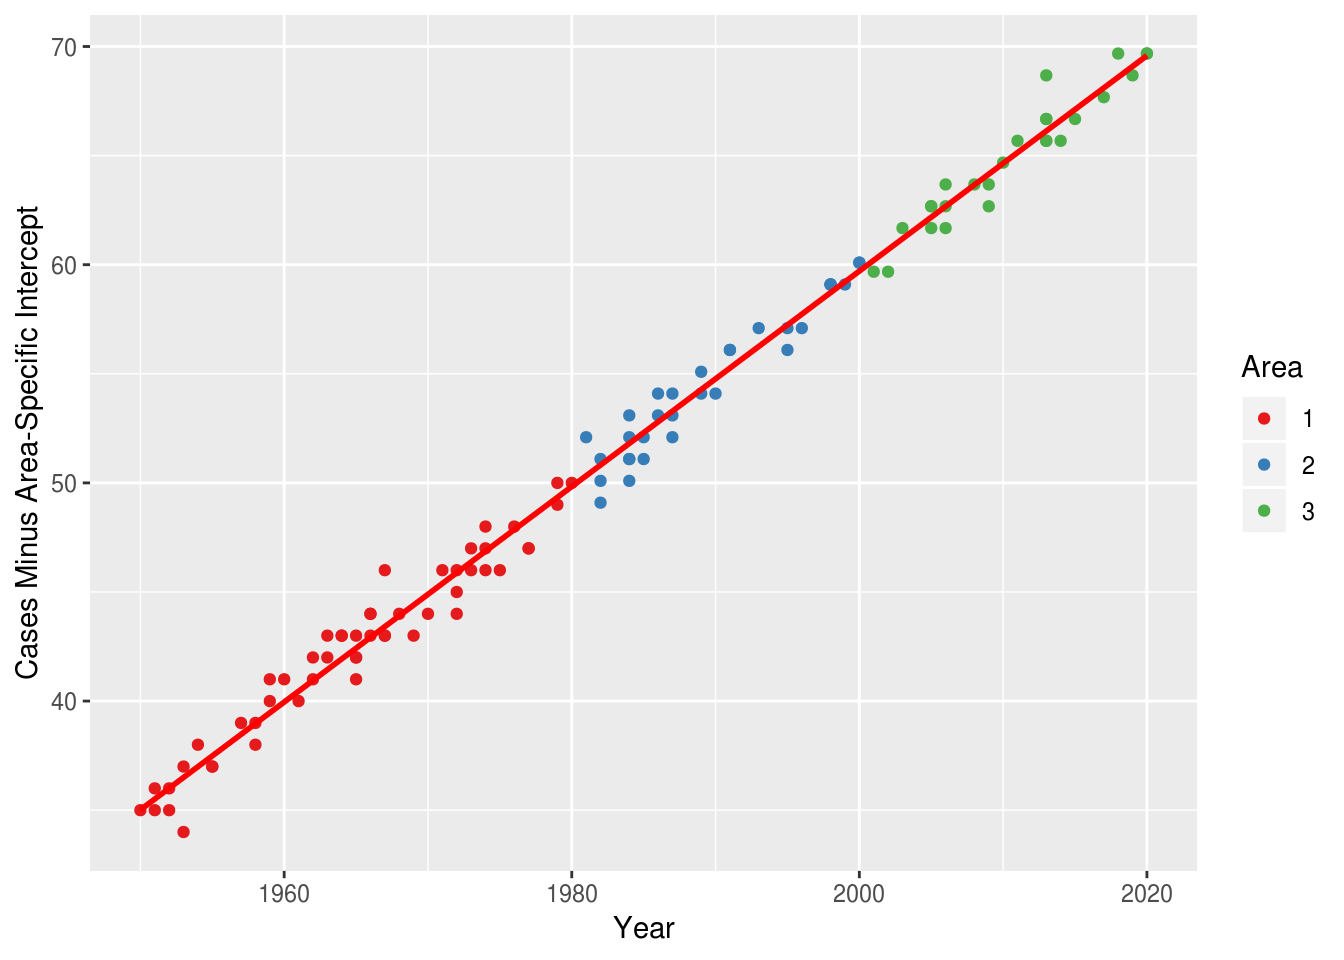
\includegraphics{website_files/figure-latex/unnamed-chunk-33-1.pdf}

\section{Applying The Regression
Models}\label{applying-the-regression-models}

So how do you obtain \texttt{area-specific\ intercepts}? If you have a
large amount of datapoints for each area, and not many areas, you can
just include \texttt{area} as a categorical variable in your regression.
These \texttt{area-specific\ intercepts} are called
\texttt{fixed\ effects}.

\begin{Shaded}
\begin{Highlighting}[]
\NormalTok{fit <-}\StringTok{ }\KeywordTok{lm}\NormalTok{(y }\OperatorTok{~}\StringTok{ }\KeywordTok{as.factor}\NormalTok{(fylke) }\OperatorTok{+}\StringTok{ }\NormalTok{yearMinus1950, }\DataTypeTok{data =}\NormalTok{ d)}
\KeywordTok{summary}\NormalTok{(fit)}
\end{Highlighting}
\end{Shaded}

\begin{verbatim}
## 
## Call:
## lm(formula = y ~ as.factor(fylke) + yearMinus1950, data = d)
## 
## Residuals:
##      Min       1Q   Median       3Q      Max 
## -2.49741 -0.50980  0.03513  0.55371  2.58931 
## 
## Coefficients:
##                    Estimate Std. Error t value Pr(>|t|)    
## (Intercept)        35.01599    0.22624  154.78   <2e-16 ***
## as.factor(fylke)2 -30.09439    0.36891  -81.58   <2e-16 ***
## as.factor(fylke)3 -59.67945    0.60794  -98.17   <2e-16 ***
## yearMinus1950       0.49381    0.01243   39.73   <2e-16 ***
## ---
## Signif. codes:  0 '***' 0.001 '**' 0.01 '*' 0.05 '.' 0.1 ' ' 1
## 
## Residual standard error: 0.9244 on 105 degrees of freedom
## Multiple R-squared:  0.9966, Adjusted R-squared:  0.9965 
## F-statistic: 1.016e+04 on 3 and 105 DF,  p-value: < 2.2e-16
\end{verbatim}

If you have few datapoints for each area, and a lot of areas, you will
need to use a \texttt{mixed\ effects} regression model, including
\texttt{random\ intercepts} for each \texttt{area}.

\begin{Shaded}
\begin{Highlighting}[]
\NormalTok{fit <-}\StringTok{ }\NormalTok{lme4}\OperatorTok{::}\KeywordTok{lmer}\NormalTok{(y }\OperatorTok{~}\StringTok{ }\NormalTok{yearMinus1950 }\OperatorTok{+}\StringTok{ }\NormalTok{(}\DecValTok{1} \OperatorTok{|}\StringTok{ }\NormalTok{fylke), }\DataTypeTok{data =}\NormalTok{ d)}
\KeywordTok{summary}\NormalTok{(fit)}
\end{Highlighting}
\end{Shaded}

\begin{verbatim}
## Linear mixed model fit by REML ['lmerMod']
## Formula: y ~ yearMinus1950 + (1 | fylke)
##    Data: d
## 
## REML criterion at convergence: 321.1
## 
## Scaled residuals: 
##      Min       1Q   Median       3Q      Max 
## -2.70424 -0.55449  0.03668  0.59846  2.80231 
## 
## Random effects:
##  Groups   Name        Variance Std.Dev.
##  fylke    (Intercept) 890.1680 29.8357 
##  Residual               0.8544  0.9244 
## Number of obs: 109, groups:  fylke, 3
## 
## Fixed effects:
##               Estimate Std. Error t value
## (Intercept)    5.10060   17.23247   0.296
## yearMinus1950  0.49357    0.01243  39.718
## 
## Correlation of Fixed Effects:
##             (Intr)
## yearMns1950 -0.028
\end{verbatim}

\begin{Shaded}
\begin{Highlighting}[]
\NormalTok{lme4}\OperatorTok{::}\KeywordTok{ranef}\NormalTok{(fit)}
\end{Highlighting}
\end{Shaded}

\begin{verbatim}
## $fylke
##   (Intercept)
## 1  29.9183802
## 2  -0.1696969
## 3 -29.7486833
\end{verbatim}

\section{Hints For Future Analyses}\label{hints-for-future-analyses-1}

In general:

\[\text{number of observations} = \text{number of time points} \times \text{number of areas}\]

So 5 years of data for aggregated Norway is worse than 5 years of data
for every municipality in Norway.

\bibliography{book.bib,packages.bib}


\end{document}
